\documentclass[1p]{elsarticle_modified}
%\bibliographystyle{elsarticle-num}

%\usepackage[colorlinks]{hyperref}
%\usepackage{abbrmath_seonhwa} %\Abb, \Ascr, \Acal ,\Abf, \Afrak
\usepackage{amsfonts}
\usepackage{amssymb}
\usepackage{amsmath}
\usepackage{amsthm}
\usepackage{scalefnt}
\usepackage{amsbsy}
\usepackage{kotex}
\usepackage{caption}
\usepackage{subfig}
\usepackage{color}
\usepackage{graphicx}
\usepackage{xcolor} %% white, black, red, green, blue, cyan, magenta, yellow
\usepackage{float}
\usepackage{setspace}
\usepackage{hyperref}

\usepackage{tikz}
\usetikzlibrary{arrows}

\usepackage{multirow}
\usepackage{array} % fixed length table
\usepackage{hhline}

%%%%%%%%%%%%%%%%%%%%%
\makeatletter
\renewcommand*\env@matrix[1][\arraystretch]{%
	\edef\arraystretch{#1}%
	\hskip -\arraycolsep
	\let\@ifnextchar\new@ifnextchar
	\array{*\c@MaxMatrixCols c}}
\makeatother %https://tex.stackexchange.com/questions/14071/how-can-i-increase-the-line-spacing-in-a-matrix
%%%%%%%%%%%%%%%

\usepackage[normalem]{ulem}

\newcommand{\msout}[1]{\ifmmode\text{\sout{\ensuremath{#1}}}\else\sout{#1}\fi}
%SOURCE: \msout is \stkout macro in https://tex.stackexchange.com/questions/20609/strikeout-in-math-mode

\newcommand{\cancel}[1]{
	\ifmmode
	{\color{red}\msout{#1}}
	\else
	{\color{red}\sout{#1}}
	\fi
}

\newcommand{\add}[1]{
	{\color{blue}\uwave{#1}}
}

\newcommand{\replace}[2]{
	\ifmmode
	{\color{red}\msout{#1}}{\color{blue}\uwave{#2}}
	\else
	{\color{red}\sout{#1}}{\color{blue}\uwave{#2}}
	\fi
}

\newcommand{\Sol}{\mathcal{S}} %segment
\newcommand{\D}{D} %diagram
\newcommand{\A}{\mathcal{A}} %arc


%%%%%%%%%%%%%%%%%%%%%%%%%%%%%5 test

\def\sl{\operatorname{\textup{SL}}(2,\Cbb)}
\def\psl{\operatorname{\textup{PSL}}(2,\Cbb)}
\def\quan{\mkern 1mu \triangleright \mkern 1mu}

\theoremstyle{definition}
\newtheorem{thm}{Theorem}[section]
\newtheorem{prop}[thm]{Proposition}
\newtheorem{lem}[thm]{Lemma}
\newtheorem{ques}[thm]{Question}
\newtheorem{cor}[thm]{Corollary}
\newtheorem{defn}[thm]{Definition}
\newtheorem{exam}[thm]{Example}
\newtheorem{rmk}[thm]{Remark}
\newtheorem{alg}[thm]{Algorithm}

\newcommand{\I}{\sqrt{-1}}
\begin{document}

%\begin{frontmatter}
%
%\title{Boundary parabolic representations of knots up to 8 crossings}
%
%%% Group authors per affiliation:
%\author{Yunhi Cho} 
%\address{Department of Mathematics, University of Seoul, Seoul, Korea}
%\ead{yhcho@uos.ac.kr}
%
%
%\author{Seonhwa Kim} %\fnref{s_kim}}
%\address{Center for Geometry and Physics, Institute for Basic Science, Pohang, 37673, Korea}
%\ead{ryeona17@ibs.re.kr}
%
%\author{Hyuk Kim}
%\address{Department of Mathematical Sciences, Seoul National University, Seoul 08826, Korea}
%\ead{hyukkim@snu.ac.kr}
%
%\author{Seokbeom Yoon}
%\address{Department of Mathematical Sciences, Seoul National University, Seoul, 08826,  Korea}
%\ead{sbyoon15@snu.ac.kr}
%
%\begin{abstract}
%We find all boundary parabolic representation of knots up to 8 crossings.
%
%\end{abstract}
%\begin{keyword}
%    \MSC[2010] 57M25 
%\end{keyword}
%
%\end{frontmatter}

%\linenumbers
%\tableofcontents
%
\newcommand\colored[1]{\textcolor{white}{\rule[-0.35ex]{0.8em}{1.4ex}}\kern-0.8em\color{red} #1}%
%\newcommand\colored[1]{\textcolor{white}{ #1}\kern-2.17ex	\textcolor{white}{ #1}\kern-1.81ex	\textcolor{white}{ #1}\kern-2.15ex\color{red}#1	}

{\Large $\underline{12a_{1211}~(K12a_{1211})}$}

\setlength{\tabcolsep}{10pt}
\renewcommand{\arraystretch}{1.6}
\vspace{1cm}\begin{tabular}{m{100pt}>{\centering\arraybackslash}m{274pt}}
\multirow{5}{120pt}{
	\centering
	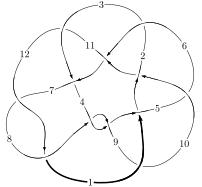
\includegraphics[width=112pt]{../../../GIT/diagram.site/Diagrams/png/2012_12a_1211.png}\\
\ \ \ A knot diagram\footnotemark}&
\allowdisplaybreaks
\textbf{Linearized knot diagam} \\
\cline{2-2}
 &
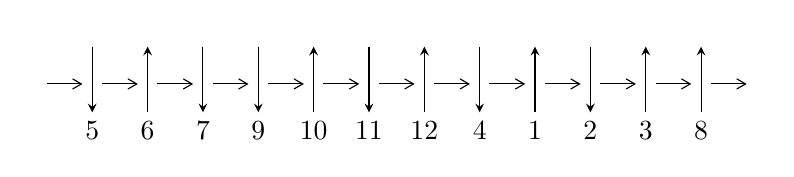
\begin{tikzpicture}[x=20pt, y=17pt]
	% nodes
	\node (C0) at (0, 0) {};
	\node (C1) at (1, 0) {};
	\node (C1U) at (1, +1) {};
	\node (C1D) at (1, -1) {5};

	\node (C2) at (2, 0) {};
	\node (C2U) at (2, +1) {};
	\node (C2D) at (2, -1) {6};

	\node (C3) at (3, 0) {};
	\node (C3U) at (3, +1) {};
	\node (C3D) at (3, -1) {7};

	\node (C4) at (4, 0) {};
	\node (C4U) at (4, +1) {};
	\node (C4D) at (4, -1) {9};

	\node (C5) at (5, 0) {};
	\node (C5U) at (5, +1) {};
	\node (C5D) at (5, -1) {10};

	\node (C6) at (6, 0) {};
	\node (C6U) at (6, +1) {};
	\node (C6D) at (6, -1) {11};

	\node (C7) at (7, 0) {};
	\node (C7U) at (7, +1) {};
	\node (C7D) at (7, -1) {12};

	\node (C8) at (8, 0) {};
	\node (C8U) at (8, +1) {};
	\node (C8D) at (8, -1) {4};

	\node (C9) at (9, 0) {};
	\node (C9U) at (9, +1) {};
	\node (C9D) at (9, -1) {1};

	\node (C10) at (10, 0) {};
	\node (C10U) at (10, +1) {};
	\node (C10D) at (10, -1) {2};

	\node (C11) at (11, 0) {};
	\node (C11U) at (11, +1) {};
	\node (C11D) at (11, -1) {3};

	\node (C12) at (12, 0) {};
	\node (C12U) at (12, +1) {};
	\node (C12D) at (12, -1) {8};
	\node (C13) at (13, 0) {};

	% arrows
	\draw[->,>={angle 60}]
	(C0) edge (C1) (C1) edge (C2) (C2) edge (C3) (C3) edge (C4) (C4) edge (C5) (C5) edge (C6) (C6) edge (C7) (C7) edge (C8) (C8) edge (C9) (C9) edge (C10) (C10) edge (C11) (C11) edge (C12) (C12) edge (C13) ;	\draw[->,>=stealth]
	(C1U) edge (C1D) (C2D) edge (C2U) (C3U) edge (C3D) (C4U) edge (C4D) (C5D) edge (C5U) (C6U) edge (C6D) (C7D) edge (C7U) (C8U) edge (C8D) (C9D) edge (C9U) (C10U) edge (C10D) (C11D) edge (C11U) (C12D) edge (C12U) ;
	\end{tikzpicture} \\
\hhline{~~} \\& 
\textbf{Solving Sequence} \\ \cline{2-2} 
 &
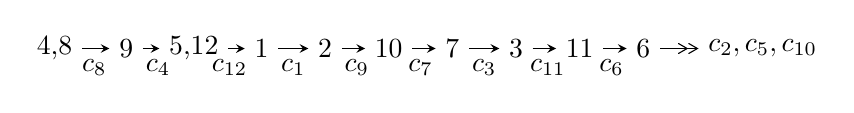
\begin{tikzpicture}[x=23pt, y=7pt]
	% node
	\node (A0) at (-1/8, 0) {4,8};
	\node (A1) at (1, 0) {9};
	\node (A2) at (33/16, 0) {5,12};
	\node (A3) at (25/8, 0) {1};
	\node (A4) at (33/8, 0) {2};
	\node (A5) at (41/8, 0) {10};
	\node (A6) at (49/8, 0) {7};
	\node (A7) at (57/8, 0) {3};
	\node (A8) at (65/8, 0) {11};
	\node (A9) at (73/8, 0) {6};
	\node (C1) at (1/2, -1) {$c_{8}$};
	\node (C2) at (3/2, -1) {$c_{4}$};
	\node (C3) at (21/8, -1) {$c_{12}$};
	\node (C4) at (29/8, -1) {$c_{1}$};
	\node (C5) at (37/8, -1) {$c_{9}$};
	\node (C6) at (45/8, -1) {$c_{7}$};
	\node (C7) at (53/8, -1) {$c_{3}$};
	\node (C8) at (61/8, -1) {$c_{11}$};
	\node (C9) at (69/8, -1) {$c_{6}$};
	\node (A10) at (11, 0) {$c_{2},c_{5},c_{10}$};

	% edge
	\draw[->,>=stealth]	
	(A0) edge (A1) (A1) edge (A2) (A2) edge (A3) (A3) edge (A4) (A4) edge (A5) (A5) edge (A6) (A6) edge (A7) (A7) edge (A8) (A8) edge (A9) ;
	\draw[->>,>={angle 60}]	
	(A9) edge (A10);
\end{tikzpicture} \\ 

\end{tabular} \\

\footnotetext{
The image of knot diagram is generated by the software ``\textbf{Draw programme}" developed by Andrew Bartholomew(\url{http://www.layer8.co.uk/maths/draw/index.htm\#Running-draw}), where we modified some parts for our purpose(\url{https://github.com/CATsTAILs/LinksPainter}).
}\phantom \\ \newline 
\centering \textbf{Ideals for irreducible components\footnotemark of $X_{\text{par}}$} 
 
\begin{align*}
I^u_{1}&=\langle 
2.75820\times10^{1048} u^{163}-3.15201\times10^{1048} u^{162}+\cdots+7.37813\times10^{1048} b-3.04580\times10^{1050},\\
\phantom{I^u_{1}}&\phantom{= \langle  }1.81233\times10^{1053} u^{163}-5.92096\times10^{1054} u^{162}+\cdots+2.02597\times10^{1055} a-4.42522\times10^{1056},\\
\phantom{I^u_{1}}&\phantom{= \langle  }u^{164}-2 u^{163}+\cdots-3386 u+61\rangle \\
I^u_{2}&=\langle 
-5.26861\times10^{16} u^{25}+2.05028\times10^{16} u^{24}+\cdots+3.42865\times10^{15} b-8.25553\times10^{16},\\
\phantom{I^u_{2}}&\phantom{= \langle  }4.92095\times10^{16} u^{25}-2.56966\times10^{16} u^{24}+\cdots+3.42865\times10^{15} a+1.11054\times10^{17},\;u^{26}- u^{25}+\cdots+23 u-1\rangle \\
I^u_{3}&=\langle 
- u^3+b+u-1,\;u^5+4 u^4- u^2+3 a+3 u+2,\;u^6- u^4+2 u^3+u^2- u+1\rangle \\
\\
\end{align*}
\raggedright * 3 irreducible components of $\dim_{\mathbb{C}}=0$, with total 196 representations.\\
\footnotetext{All coefficients of polynomials are rational numbers. But the coefficients are sometimes approximated in decimal forms when there is not enough margin.}
\newpage
\renewcommand{\arraystretch}{1}
\centering \section*{I. $I^u_{1}= \langle 2.76\times10^{1048} u^{163}-3.15\times10^{1048} u^{162}+\cdots+7.38\times10^{1048} b-3.05\times10^{1050},\;1.81\times10^{1053} u^{163}-5.92\times10^{1054} u^{162}+\cdots+2.03\times10^{1055} a-4.43\times10^{1056},\;u^{164}-2 u^{163}+\cdots-3386 u+61 \rangle$}
\flushleft \textbf{(i) Arc colorings}\\
\begin{tabular}{m{7pt} m{180pt} m{7pt} m{180pt} }
\flushright $a_{4}=$&$\begin{pmatrix}0\\u\end{pmatrix}$ \\
\flushright $a_{8}=$&$\begin{pmatrix}1\\0\end{pmatrix}$ \\
\flushright $a_{9}=$&$\begin{pmatrix}1\\u^2\end{pmatrix}$ \\
\flushright $a_{5}=$&$\begin{pmatrix}- u\\- u^3+u\end{pmatrix}$ \\
\flushright $a_{12}=$&$\begin{pmatrix}-0.00894549 u^{163}+0.292253 u^{162}+\cdots+398.496 u+21.8424\\-0.373834 u^{163}+0.427210 u^{162}+\cdots-2124.70 u+41.2815\end{pmatrix}$ \\
\flushright $a_{1}=$&$\begin{pmatrix}-0.382780 u^{163}+0.719463 u^{162}+\cdots-1726.20 u+63.1239\\-0.373834 u^{163}+0.427210 u^{162}+\cdots-2124.70 u+41.2815\end{pmatrix}$ \\
\flushright $a_{2}=$&$\begin{pmatrix}-0.104186 u^{163}+0.429492 u^{162}+\cdots-498.173 u+40.4408\\-0.441826 u^{163}+0.511079 u^{162}+\cdots-2464.92 u+47.6643\end{pmatrix}$ \\
\flushright $a_{10}=$&$\begin{pmatrix}-0.171894 u^{163}+0.144356 u^{162}+\cdots+465.124 u-54.8742\\0.158864 u^{163}-0.326697 u^{162}+\cdots-480.252 u+6.26403\end{pmatrix}$ \\
\flushright $a_{7}=$&$\begin{pmatrix}0.246697 u^{163}-0.380836 u^{162}+\cdots-1682.95 u+77.4279\\0.100974 u^{163}-0.192003 u^{162}+\cdots+873.840 u-13.7367\end{pmatrix}$ \\
\flushright $a_{3}=$&$\begin{pmatrix}-0.366074 u^{163}+0.741373 u^{162}+\cdots-1622.52 u+83.2336\\0.283184 u^{163}-0.109775 u^{162}+\cdots+1197.22 u-18.3804\end{pmatrix}$ \\
\flushright $a_{11}=$&$\begin{pmatrix}-0.142442 u^{163}+0.0702581 u^{162}+\cdots-583.910 u-17.2748\\0.105327 u^{163}-0.196052 u^{162}+\cdots-774.839 u+12.9511\end{pmatrix}$ \\
\flushright $a_{6}=$&$\begin{pmatrix}1.01159 u^{163}-2.64363 u^{162}+\cdots-2987.89 u+108.144\\-0.176189 u^{163}+0.321162 u^{162}+\cdots+544.973 u-7.21403\end{pmatrix}$\\&\end{tabular}
\flushleft \textbf{(ii) Obstruction class $= -1$}\\~\\
\flushleft \textbf{(iii) Cusp Shapes $= 0.183937 u^{163}+1.47453 u^{162}+\cdots-1344.67 u+46.8656$}\\~\\
\newpage\renewcommand{\arraystretch}{1}
\flushleft \textbf{(iv) u-Polynomials at the component}\newline \\
\begin{tabular}{m{50pt}|m{274pt}}
Crossings & \hspace{64pt}u-Polynomials at each crossing \\
\hline $$\begin{aligned}c_{1}\end{aligned}$$&$\begin{aligned}
&u^{164}+7 u^{163}+\cdots-114622 u-349484
\end{aligned}$\\
\hline $$\begin{aligned}c_{2}\end{aligned}$$&$\begin{aligned}
&u^{164}+2 u^{163}+\cdots-173301 u+10677
\end{aligned}$\\
\hline $$\begin{aligned}c_{3}\end{aligned}$$&$\begin{aligned}
&3(3 u^{164}+30 u^{163}+\cdots-23 u-1)
\end{aligned}$\\
\hline $$\begin{aligned}c_{4},c_{8}\end{aligned}$$&$\begin{aligned}
&u^{164}-2 u^{163}+\cdots-3386 u+61
\end{aligned}$\\
\hline $$\begin{aligned}c_{5}\end{aligned}$$&$\begin{aligned}
&3(3 u^{164}-14 u^{162}+\cdots+3228 u+43)
\end{aligned}$\\
\hline $$\begin{aligned}c_{6}\end{aligned}$$&$\begin{aligned}
&3(3 u^{164}-14 u^{162}+\cdots-3228 u+43)
\end{aligned}$\\
\hline $$\begin{aligned}c_{7},c_{12}\end{aligned}$$&$\begin{aligned}
&u^{164}+2 u^{163}+\cdots+3386 u+61
\end{aligned}$\\
\hline $$\begin{aligned}c_{9}\end{aligned}$$&$\begin{aligned}
&3(3 u^{164}-30 u^{163}+\cdots+23 u-1)
\end{aligned}$\\
\hline $$\begin{aligned}c_{10}\end{aligned}$$&$\begin{aligned}
&u^{164}-2 u^{163}+\cdots+173301 u+10677
\end{aligned}$\\
\hline $$\begin{aligned}c_{11}\end{aligned}$$&$\begin{aligned}
&u^{164}-7 u^{163}+\cdots+114622 u-349484
\end{aligned}$\\
\hline
\end{tabular}\\~\\
\newpage\renewcommand{\arraystretch}{1}
\flushleft \textbf{(v) Riley Polynomials at the component}\newline \\
\begin{tabular}{m{50pt}|m{274pt}}
Crossings & \hspace{64pt}Riley Polynomials at each crossing \\
\hline $$\begin{aligned}c_{1},c_{11}\end{aligned}$$&$\begin{aligned}
&y^{164}-41 y^{163}+\cdots-4668550960796 y+122139066256
\end{aligned}$\\
\hline $$\begin{aligned}c_{2},c_{10}\end{aligned}$$&$\begin{aligned}
&y^{164}-34 y^{163}+\cdots-9384110787 y+113998329
\end{aligned}$\\
\hline $$\begin{aligned}c_{3},c_{9}\end{aligned}$$&$\begin{aligned}
&9(9 y^{164}+168 y^{163}+\cdots-3213 y+1)
\end{aligned}$\\
\hline $$\begin{aligned}c_{4},c_{7},c_{8}\\c_{12}\end{aligned}$$&$\begin{aligned}
&y^{164}-110 y^{163}+\cdots-5163208 y+3721
\end{aligned}$\\
\hline $$\begin{aligned}c_{5},c_{6}\end{aligned}$$&$\begin{aligned}
&9(9 y^{164}-84 y^{163}+\cdots-1.13525\times10^{7} y+1849)
\end{aligned}$\\
\hline
\end{tabular}\\~\\
\newpage\flushleft \textbf{(vi) Complex Volumes and Cusp Shapes}
$$\begin{array}{c|c|c}  
\text{Solutions to }I^u_{1}& \I (\text{vol} + \sqrt{-1}CS) & \text{Cusp shape}\\
 \hline 
\begin{aligned}
u &= \phantom{-}0.798897 + 0.600859 I \\
a &= -1.58652 - 1.10809 I \\
b &= \phantom{-}1.043510 - 0.483445 I\end{aligned}
 & \phantom{-}0.39756 - 4.84593 I & \phantom{-0.000000 } 0 \\ \hline\begin{aligned}
u &= \phantom{-}0.798897 - 0.600859 I \\
a &= -1.58652 + 1.10809 I \\
b &= \phantom{-}1.043510 + 0.483445 I\end{aligned}
 & \phantom{-}0.39756 + 4.84593 I & \phantom{-0.000000 } 0 \\ \hline\begin{aligned}
u &= -0.763806 + 0.635007 I \\
a &= \phantom{-}1.25065 - 0.72745 I \\
b &= -0.763806 - 0.635007 I\end{aligned}
 & \phantom{-0.000000 -}3.87653 I & \phantom{-0.000000 } 0 \\ \hline\begin{aligned}
u &= -0.763806 - 0.635007 I \\
a &= \phantom{-}1.25065 + 0.72745 I \\
b &= -0.763806 + 0.635007 I\end{aligned}
 & \phantom{-0.000000 } -3.87653 I & \phantom{-0.000000 } 0 \\ \hline\begin{aligned}
u &= -0.936998 + 0.373525 I \\
a &= \phantom{-}0.930907 - 0.791991 I \\
b &= -1.42614 - 0.93512 I\end{aligned}
 & \phantom{-}2.66702 + 4.07987 I & \phantom{-0.000000 } 0 \\ \hline\begin{aligned}
u &= -0.936998 - 0.373525 I \\
a &= \phantom{-}0.930907 + 0.791991 I \\
b &= -1.42614 + 0.93512 I\end{aligned}
 & \phantom{-}2.66702 - 4.07987 I & \phantom{-0.000000 } 0 \\ \hline\begin{aligned}
u &= -1.011230 + 0.030403 I \\
a &= -0.89458 + 2.35109 I \\
b &= \phantom{-}1.090610 + 0.363390 I\end{aligned}
 & -0.175281 + 0.663751 I & \phantom{-0.000000 } 0 \\ \hline\begin{aligned}
u &= -1.011230 - 0.030403 I \\
a &= -0.89458 - 2.35109 I \\
b &= \phantom{-}1.090610 - 0.363390 I\end{aligned}
 & -0.175281 - 0.663751 I & \phantom{-0.000000 } 0 \\ \hline\begin{aligned}
u &= -0.977792 + 0.007736 I \\
a &= \phantom{-}0.51300 - 3.04293 I \\
b &= -0.977792 - 0.007736 I\end{aligned}
 & \phantom{-0.000000 } -0.507463 I & \phantom{-0.000000 } 0 \\ \hline\begin{aligned}
u &= -0.977792 - 0.007736 I \\
a &= \phantom{-}0.51300 + 3.04293 I \\
b &= -0.977792 + 0.007736 I\end{aligned}
 & \phantom{-0.000000 -}0.507463 I & \phantom{-0.000000 } 0\\
 \hline 
 \end{array}$$\newpage$$\begin{array}{c|c|c}  
\text{Solutions to }I^u_{1}& \I (\text{vol} + \sqrt{-1}CS) & \text{Cusp shape}\\
 \hline 
\begin{aligned}
u &= -0.960617 + 0.124105 I \\
a &= \phantom{-}0.235681 - 0.341648 I \\
b &= \phantom{-}0.365350 - 0.710425 I\end{aligned}
 & -1.70988 + 0.60280 I & \phantom{-0.000000 } 0 \\ \hline\begin{aligned}
u &= -0.960617 - 0.124105 I \\
a &= \phantom{-}0.235681 + 0.341648 I \\
b &= \phantom{-}0.365350 + 0.710425 I\end{aligned}
 & -1.70988 - 0.60280 I & \phantom{-0.000000 } 0 \\ \hline\begin{aligned}
u &= -1.032720 + 0.065105 I \\
a &= \phantom{-}0.953281 + 0.485959 I \\
b &= -1.46278 + 0.53288 I\end{aligned}
 & -2.74159 + 0.88861 I & \phantom{-0.000000 } 0 \\ \hline\begin{aligned}
u &= -1.032720 - 0.065105 I \\
a &= \phantom{-}0.953281 - 0.485959 I \\
b &= -1.46278 - 0.53288 I\end{aligned}
 & -2.74159 - 0.88861 I & \phantom{-0.000000 } 0 \\ \hline\begin{aligned}
u &= \phantom{-}0.963273\phantom{ +0.000000I} \\
a &= -1.20577\phantom{ +0.000000I} \\
b &= \phantom{-}2.02298\phantom{ +0.000000I}\end{aligned}
 & \phantom{-}3.88198\phantom{ +0.000000I} & \phantom{-0.000000 } 0 \\ \hline\begin{aligned}
u &= \phantom{-}0.949425 + 0.120762 I \\
a &= \phantom{-}0.175869 + 0.128372 I \\
b &= \phantom{-}0.07698 + 1.55742 I\end{aligned}
 & -0.78508 - 5.40731 I & \phantom{-0.000000 } 0 \\ \hline\begin{aligned}
u &= \phantom{-}0.949425 - 0.120762 I \\
a &= \phantom{-}0.175869 - 0.128372 I \\
b &= \phantom{-}0.07698 - 1.55742 I\end{aligned}
 & -0.78508 + 5.40731 I & \phantom{-0.000000 } 0 \\ \hline\begin{aligned}
u &= -0.006754 + 1.046690 I \\
a &= -1.52430 - 0.32954 I \\
b &= \phantom{-}1.331860 + 0.369170 I\end{aligned}
 & \phantom{-}7.13952 + 6.54845 I & \phantom{-0.000000 } 0 \\ \hline\begin{aligned}
u &= -0.006754 - 1.046690 I \\
a &= -1.52430 + 0.32954 I \\
b &= \phantom{-}1.331860 - 0.369170 I\end{aligned}
 & \phantom{-}7.13952 - 6.54845 I & \phantom{-0.000000 } 0 \\ \hline\begin{aligned}
u &= \phantom{-}0.086283 + 1.047630 I \\
a &= -1.59143 - 0.00241 I \\
b &= \phantom{-}1.356670 - 0.282535 I\end{aligned}
 & \phantom{-}7.20749 - 6.27464 I & \phantom{-0.000000 } 0\\
 \hline 
 \end{array}$$\newpage$$\begin{array}{c|c|c}  
\text{Solutions to }I^u_{1}& \I (\text{vol} + \sqrt{-1}CS) & \text{Cusp shape}\\
 \hline 
\begin{aligned}
u &= \phantom{-}0.086283 - 1.047630 I \\
a &= -1.59143 + 0.00241 I \\
b &= \phantom{-}1.356670 + 0.282535 I\end{aligned}
 & \phantom{-}7.20749 + 6.27464 I & \phantom{-0.000000 } 0 \\ \hline\begin{aligned}
u &= \phantom{-}1.074770 + 0.100746 I \\
a &= \phantom{-}0.394734 - 0.610938 I \\
b &= -0.98104 - 1.33165 I\end{aligned}
 & -2.11600 - 5.55049 I & \phantom{-0.000000 } 0 \\ \hline\begin{aligned}
u &= \phantom{-}1.074770 - 0.100746 I \\
a &= \phantom{-}0.394734 + 0.610938 I \\
b &= -0.98104 + 1.33165 I\end{aligned}
 & -2.11600 + 5.55049 I & \phantom{-0.000000 } 0 \\ \hline\begin{aligned}
u &= -0.984874 + 0.458102 I \\
a &= -0.0748509 - 0.1043720 I \\
b &= \phantom{-}0.554699 - 0.592619 I\end{aligned}
 & -1.040880 + 0.811517 I & \phantom{-0.000000 } 0 \\ \hline\begin{aligned}
u &= -0.984874 - 0.458102 I \\
a &= -0.0748509 + 0.1043720 I \\
b &= \phantom{-}0.554699 + 0.592619 I\end{aligned}
 & -1.040880 - 0.811517 I & \phantom{-0.000000 } 0 \\ \hline\begin{aligned}
u &= -1.076700 + 0.166906 I \\
a &= \phantom{-}1.56634 - 0.94640 I \\
b &= -1.349670 - 0.408498 I\end{aligned}
 & -3.03570 + 3.98628 I & \phantom{-0.000000 } 0 \\ \hline\begin{aligned}
u &= -1.076700 - 0.166906 I \\
a &= \phantom{-}1.56634 + 0.94640 I \\
b &= -1.349670 + 0.408498 I\end{aligned}
 & -3.03570 - 3.98628 I & \phantom{-0.000000 } 0 \\ \hline\begin{aligned}
u &= \phantom{-}0.986695 + 0.502565 I \\
a &= -0.61025 - 1.29255 I \\
b &= \phantom{-}1.149870 - 0.134063 I\end{aligned}
 & \phantom{-}4.53081 - 4.33380 I & \phantom{-0.000000 } 0 \\ \hline\begin{aligned}
u &= \phantom{-}0.986695 - 0.502565 I \\
a &= -0.61025 + 1.29255 I \\
b &= \phantom{-}1.149870 + 0.134063 I\end{aligned}
 & \phantom{-}4.53081 + 4.33380 I & \phantom{-0.000000 } 0 \\ \hline\begin{aligned}
u &= -0.195421 + 1.097560 I \\
a &= \phantom{-}1.82772 + 0.41740 I \\
b &= -1.345620 - 0.053192 I\end{aligned}
 & \phantom{-}5.56120 - 5.11329 I & \phantom{-0.000000 } 0\\
 \hline 
 \end{array}$$\newpage$$\begin{array}{c|c|c}  
\text{Solutions to }I^u_{1}& \I (\text{vol} + \sqrt{-1}CS) & \text{Cusp shape}\\
 \hline 
\begin{aligned}
u &= -0.195421 - 1.097560 I \\
a &= \phantom{-}1.82772 - 0.41740 I \\
b &= -1.345620 + 0.053192 I\end{aligned}
 & \phantom{-}5.56120 + 5.11329 I & \phantom{-0.000000 } 0 \\ \hline\begin{aligned}
u &= -0.470115 + 0.743651 I \\
a &= \phantom{-}0.665886 - 0.437045 I \\
b &= \phantom{-}0.091710 + 0.211062 I\end{aligned}
 & -1.99149 + 2.63914 I & \phantom{-0.000000 } 0 \\ \hline\begin{aligned}
u &= -0.470115 - 0.743651 I \\
a &= \phantom{-}0.665886 + 0.437045 I \\
b &= \phantom{-}0.091710 - 0.211062 I\end{aligned}
 & -1.99149 - 2.63914 I & \phantom{-0.000000 } 0 \\ \hline\begin{aligned}
u &= -0.856505 + 0.197199 I \\
a &= \phantom{-}1.44080 - 0.04041 I \\
b &= \phantom{-}0.298357 - 0.180165 I\end{aligned}
 & -0.687738 - 0.103671 I & \phantom{-0.000000 } 0 \\ \hline\begin{aligned}
u &= -0.856505 - 0.197199 I \\
a &= \phantom{-}1.44080 + 0.04041 I \\
b &= \phantom{-}0.298357 + 0.180165 I\end{aligned}
 & -0.687738 + 0.103671 I & \phantom{-0.000000 } 0 \\ \hline\begin{aligned}
u &= \phantom{-}0.461785 + 1.023910 I \\
a &= -0.520857 + 0.245986 I \\
b &= \phantom{-}0.342421 + 0.075790 I\end{aligned}
 & \phantom{-}0.33309 + 5.06568 I & \phantom{-0.000000 } 0 \\ \hline\begin{aligned}
u &= \phantom{-}0.461785 - 1.023910 I \\
a &= -0.520857 - 0.245986 I \\
b &= \phantom{-}0.342421 - 0.075790 I\end{aligned}
 & \phantom{-}0.33309 - 5.06568 I & \phantom{-0.000000 } 0 \\ \hline\begin{aligned}
u &= -0.423919 + 0.764806 I \\
a &= -0.203308 + 0.416945 I \\
b &= -0.008003 - 0.519204 I\end{aligned}
 & -1.68748 + 2.68990 I & \phantom{-0.000000 } 0 \\ \hline\begin{aligned}
u &= -0.423919 - 0.764806 I \\
a &= -0.203308 - 0.416945 I \\
b &= -0.008003 + 0.519204 I\end{aligned}
 & -1.68748 - 2.68990 I & \phantom{-0.000000 } 0 \\ \hline\begin{aligned}
u &= \phantom{-}0.860890 + 0.108703 I \\
a &= -0.73831 - 1.48618 I \\
b &= \phantom{-}0.993044 - 0.804227 I\end{aligned}
 & \phantom{-}0.34989 - 4.29120 I & \phantom{-0.000000 } 0\\
 \hline 
 \end{array}$$\newpage$$\begin{array}{c|c|c}  
\text{Solutions to }I^u_{1}& \I (\text{vol} + \sqrt{-1}CS) & \text{Cusp shape}\\
 \hline 
\begin{aligned}
u &= \phantom{-}0.860890 - 0.108703 I \\
a &= -0.73831 + 1.48618 I \\
b &= \phantom{-}0.993044 + 0.804227 I\end{aligned}
 & \phantom{-}0.34989 + 4.29120 I & \phantom{-0.000000 } 0 \\ \hline\begin{aligned}
u &= \phantom{-}1.13423\phantom{ +0.000000I} \\
a &= \phantom{-}0.110542\phantom{ +0.000000I} \\
b &= -1.44475\phantom{ +0.000000I}\end{aligned}
 & \phantom{-}3.38142\phantom{ +0.000000I} & \phantom{-0.000000 } 0 \\ \hline\begin{aligned}
u &= \phantom{-}1.137900 + 0.144896 I \\
a &= \phantom{-}1.23584 + 1.28400 I \\
b &= -1.285350 + 0.556809 I\end{aligned}
 & -2.07933 - 10.92060 I & \phantom{-0.000000 } 0 \\ \hline\begin{aligned}
u &= \phantom{-}1.137900 - 0.144896 I \\
a &= \phantom{-}1.23584 - 1.28400 I \\
b &= -1.285350 - 0.556809 I\end{aligned}
 & -2.07933 + 10.92060 I & \phantom{-0.000000 } 0 \\ \hline\begin{aligned}
u &= \phantom{-}0.847347 + 0.086135 I \\
a &= \phantom{-}0.96361 - 1.68719 I \\
b &= -0.646360 - 0.016081 I\end{aligned}
 & \phantom{-}1.44457 - 2.68465 I & \phantom{-0.000000 } 0 \\ \hline\begin{aligned}
u &= \phantom{-}0.847347 - 0.086135 I \\
a &= \phantom{-}0.96361 + 1.68719 I \\
b &= -0.646360 + 0.016081 I\end{aligned}
 & \phantom{-}1.44457 + 2.68465 I & \phantom{-0.000000 } 0 \\ \hline\begin{aligned}
u &= \phantom{-}1.090610 + 0.363390 I \\
a &= \phantom{-}0.98490 + 2.18329 I \\
b &= -1.011230 + 0.030403 I\end{aligned}
 & \phantom{-}0.175281 - 0.663751 I & \phantom{-0.000000 } 0 \\ \hline\begin{aligned}
u &= \phantom{-}1.090610 - 0.363390 I \\
a &= \phantom{-}0.98490 - 2.18329 I \\
b &= -1.011230 - 0.030403 I\end{aligned}
 & \phantom{-}0.175281 + 0.663751 I & \phantom{-0.000000 } 0 \\ \hline\begin{aligned}
u &= \phantom{-}1.043510 + 0.483445 I \\
a &= -0.99622 - 1.06959 I \\
b &= \phantom{-}0.798897 - 0.600859 I\end{aligned}
 & -0.39756 - 4.84593 I & \phantom{-0.000000 } 0 \\ \hline\begin{aligned}
u &= \phantom{-}1.043510 - 0.483445 I \\
a &= -0.99622 + 1.06959 I \\
b &= \phantom{-}0.798897 + 0.600859 I\end{aligned}
 & -0.39756 + 4.84593 I & \phantom{-0.000000 } 0\\
 \hline 
 \end{array}$$\newpage$$\begin{array}{c|c|c}  
\text{Solutions to }I^u_{1}& \I (\text{vol} + \sqrt{-1}CS) & \text{Cusp shape}\\
 \hline 
\begin{aligned}
u &= \phantom{-}1.149870 + 0.134063 I \\
a &= -1.18567 - 0.85008 I \\
b &= \phantom{-}0.986695 - 0.502565 I\end{aligned}
 & -4.53081 - 4.33380 I & \phantom{-0.000000 } 0 \\ \hline\begin{aligned}
u &= \phantom{-}1.149870 - 0.134063 I \\
a &= -1.18567 + 0.85008 I \\
b &= \phantom{-}0.986695 + 0.502565 I\end{aligned}
 & -4.53081 + 4.33380 I & \phantom{-0.000000 } 0 \\ \hline\begin{aligned}
u &= \phantom{-}0.152711 + 0.817611 I \\
a &= -1.46956 - 0.71080 I \\
b &= \phantom{-}1.376660 + 0.150410 I\end{aligned}
 & \phantom{-}7.63231 + 0.40560 I & \phantom{-0.000000 } 0 \\ \hline\begin{aligned}
u &= \phantom{-}0.152711 - 0.817611 I \\
a &= -1.46956 + 0.71080 I \\
b &= \phantom{-}1.376660 - 0.150410 I\end{aligned}
 & \phantom{-}7.63231 - 0.40560 I & \phantom{-0.000000 } 0 \\ \hline\begin{aligned}
u &= \phantom{-}0.554699 + 0.592619 I \\
a &= \phantom{-}0.944174 + 0.625081 I \\
b &= -0.984874 - 0.458102 I\end{aligned}
 & \phantom{-}1.040880 + 0.811517 I & \phantom{-0.000000 } 0 \\ \hline\begin{aligned}
u &= \phantom{-}0.554699 - 0.592619 I \\
a &= \phantom{-}0.944174 - 0.625081 I \\
b &= -0.984874 + 0.458102 I\end{aligned}
 & \phantom{-}1.040880 - 0.811517 I & \phantom{-0.000000 } 0 \\ \hline\begin{aligned}
u &= -1.195730 + 0.036298 I \\
a &= -0.752787 + 0.321987 I \\
b &= \phantom{-}1.32024 + 0.56199 I\end{aligned}
 & -3.50885 - 0.54323 I & \phantom{-0.000000 } 0 \\ \hline\begin{aligned}
u &= -1.195730 - 0.036298 I \\
a &= -0.752787 - 0.321987 I \\
b &= \phantom{-}1.32024 - 0.56199 I\end{aligned}
 & -3.50885 + 0.54323 I & \phantom{-0.000000 } 0 \\ \hline\begin{aligned}
u &= \phantom{-}1.171860 + 0.240590 I \\
a &= -0.127633 - 0.562139 I \\
b &= -0.041618 - 1.288840 I\end{aligned}
 & -1.68961 - 5.60069 I & \phantom{-0.000000 } 0 \\ \hline\begin{aligned}
u &= \phantom{-}1.171860 - 0.240590 I \\
a &= -0.127633 + 0.562139 I \\
b &= -0.041618 + 1.288840 I\end{aligned}
 & -1.68961 + 5.60069 I & \phantom{-0.000000 } 0\\
 \hline 
 \end{array}$$\newpage$$\begin{array}{c|c|c}  
\text{Solutions to }I^u_{1}& \I (\text{vol} + \sqrt{-1}CS) & \text{Cusp shape}\\
 \hline 
\begin{aligned}
u &= \phantom{-}0.365350 + 0.710425 I \\
a &= \phantom{-}1.46386 + 0.12391 I \\
b &= -0.960617 - 0.124105 I\end{aligned}
 & \phantom{-}1.70988 + 0.60280 I & \phantom{-0.000000 } 0 \\ \hline\begin{aligned}
u &= \phantom{-}0.365350 - 0.710425 I \\
a &= \phantom{-}1.46386 - 0.12391 I \\
b &= -0.960617 + 0.124105 I\end{aligned}
 & \phantom{-}1.70988 - 0.60280 I & \phantom{-0.000000 } 0 \\ \hline\begin{aligned}
u &= -1.191000 + 0.205828 I \\
a &= -0.108582 + 0.243410 I \\
b &= \phantom{-}0.02588 + 1.63730 I\end{aligned}
 & -1.51448 + 4.61341 I & \phantom{-0.000000 } 0 \\ \hline\begin{aligned}
u &= -1.191000 - 0.205828 I \\
a &= -0.108582 - 0.243410 I \\
b &= \phantom{-}0.02588 - 1.63730 I\end{aligned}
 & -1.51448 - 4.61341 I & \phantom{-0.000000 } 0 \\ \hline\begin{aligned}
u &= \phantom{-}0.976181 + 0.729701 I \\
a &= -1.82156 - 0.88207 I \\
b &= \phantom{-}1.228230 - 0.252391 I\end{aligned}
 & \phantom{-}0.75099 - 4.04184 I & \phantom{-0.000000 } 0 \\ \hline\begin{aligned}
u &= \phantom{-}0.976181 - 0.729701 I \\
a &= -1.82156 + 0.88207 I \\
b &= \phantom{-}1.228230 + 0.252391 I\end{aligned}
 & \phantom{-}0.75099 + 4.04184 I & \phantom{-0.000000 } 0 \\ \hline\begin{aligned}
u &= \phantom{-}1.135540 + 0.459031 I \\
a &= \phantom{-}0.933898 + 0.738372 I \\
b &= -1.45784 + 0.57451 I\end{aligned}
 & \phantom{-}4.73064 - 5.03536 I & \phantom{-0.000000 } 0 \\ \hline\begin{aligned}
u &= \phantom{-}1.135540 - 0.459031 I \\
a &= \phantom{-}0.933898 - 0.738372 I \\
b &= -1.45784 - 0.57451 I\end{aligned}
 & \phantom{-}4.73064 + 5.03536 I & \phantom{-0.000000 } 0 \\ \hline\begin{aligned}
u &= -0.499041 + 1.144160 I \\
a &= \phantom{-}1.156510 - 0.558752 I \\
b &= -1.254280 + 0.319827 I\end{aligned}
 & \phantom{-}5.34717 - 6.30857 I & \phantom{-0.000000 } 0 \\ \hline\begin{aligned}
u &= -0.499041 - 1.144160 I \\
a &= \phantom{-}1.156510 + 0.558752 I \\
b &= -1.254280 - 0.319827 I\end{aligned}
 & \phantom{-}5.34717 + 6.30857 I & \phantom{-0.000000 } 0\\
 \hline 
 \end{array}$$\newpage$$\begin{array}{c|c|c}  
\text{Solutions to }I^u_{1}& \I (\text{vol} + \sqrt{-1}CS) & \text{Cusp shape}\\
 \hline 
\begin{aligned}
u &= \phantom{-}1.228230 + 0.252391 I \\
a &= -0.441495 - 1.163440 I \\
b &= \phantom{-}0.976181 - 0.729701 I\end{aligned}
 & -0.75099 - 4.04184 I & \phantom{-0.000000 } 0 \\ \hline\begin{aligned}
u &= \phantom{-}1.228230 - 0.252391 I \\
a &= -0.441495 + 1.163440 I \\
b &= \phantom{-}0.976181 + 0.729701 I\end{aligned}
 & -0.75099 + 4.04184 I & \phantom{-0.000000 } 0 \\ \hline\begin{aligned}
u &= -1.089670 + 0.631278 I \\
a &= -1.25503 + 0.72769 I \\
b &= \phantom{-}1.39299 + 0.63362 I\end{aligned}
 & \phantom{-}3.36423 + 12.46140 I & \phantom{-0.000000 } 0 \\ \hline\begin{aligned}
u &= -1.089670 - 0.631278 I \\
a &= -1.25503 - 0.72769 I \\
b &= \phantom{-}1.39299 - 0.63362 I\end{aligned}
 & \phantom{-}3.36423 - 12.46140 I & \phantom{-0.000000 } 0 \\ \hline\begin{aligned}
u &= \phantom{-}0.712768 + 0.194411 I \\
a &= \phantom{-}0.17258 + 2.03656 I \\
b &= \phantom{-}0.712768 - 0.194411 I\end{aligned}
 & \phantom{-0.000000 } -10.3096 I & \phantom{-0.000000 } 0 \\ \hline\begin{aligned}
u &= \phantom{-}0.712768 - 0.194411 I \\
a &= \phantom{-}0.17258 - 2.03656 I \\
b &= \phantom{-}0.712768 + 0.194411 I\end{aligned}
 & \phantom{-0.000000 -}10.3096 I & \phantom{-0.000000 } 0 \\ \hline\begin{aligned}
u &= \phantom{-}0.993044 + 0.804227 I \\
a &= -1.24226 - 0.95166 I \\
b &= \phantom{-}0.860890 - 0.108703 I\end{aligned}
 & -0.34989 - 4.29120 I & \phantom{-0.000000 } 0 \\ \hline\begin{aligned}
u &= \phantom{-}0.993044 - 0.804227 I \\
a &= -1.24226 + 0.95166 I \\
b &= \phantom{-}0.860890 + 0.108703 I\end{aligned}
 & -0.34989 + 4.29120 I & \phantom{-0.000000 } 0 \\ \hline\begin{aligned}
u &= \phantom{-}0.290001 + 0.656433 I \\
a &= \phantom{-}1.64742 - 0.02995 I \\
b &= -1.48126 + 0.20586 I\end{aligned}
 & \phantom{-}6.36504 - 0.06325 I & \phantom{-0.000000 } 0 \\ \hline\begin{aligned}
u &= \phantom{-}0.290001 - 0.656433 I \\
a &= \phantom{-}1.64742 + 0.02995 I \\
b &= -1.48126 - 0.20586 I\end{aligned}
 & \phantom{-}6.36504 + 0.06325 I & \phantom{-0.000000 } 0\\
 \hline 
 \end{array}$$\newpage$$\begin{array}{c|c|c}  
\text{Solutions to }I^u_{1}& \I (\text{vol} + \sqrt{-1}CS) & \text{Cusp shape}\\
 \hline 
\begin{aligned}
u &= -0.041618 + 1.288840 I \\
a &= -1.70660 + 0.24675 I \\
b &= \phantom{-}1.171860 - 0.240590 I\end{aligned}
 & \phantom{-}1.68961 - 5.60069 I & \phantom{-0.000000 } 0 \\ \hline\begin{aligned}
u &= -0.041618 - 1.288840 I \\
a &= -1.70660 - 0.24675 I \\
b &= \phantom{-}1.171860 + 0.240590 I\end{aligned}
 & \phantom{-}1.68961 + 5.60069 I & \phantom{-0.000000 } 0 \\ \hline\begin{aligned}
u &= -1.254280 + 0.319827 I \\
a &= \phantom{-}0.239759 + 0.067016 I \\
b &= -0.499041 + 1.144160 I\end{aligned}
 & -5.34717 + 6.30857 I & \phantom{-0.000000 } 0 \\ \hline\begin{aligned}
u &= -1.254280 - 0.319827 I \\
a &= \phantom{-}0.239759 - 0.067016 I \\
b &= -0.499041 - 1.144160 I\end{aligned}
 & -5.34717 - 6.30857 I & \phantom{-0.000000 } 0 \\ \hline\begin{aligned}
u &= -0.498755 + 0.469217 I \\
a &= -0.278879 + 1.118990 I \\
b &= \phantom{-}1.49497 - 0.31440 I\end{aligned}
 & \phantom{-}3.83945 - 0.42852 I & \phantom{-0.000000 } 0 \\ \hline\begin{aligned}
u &= -0.498755 - 0.469217 I \\
a &= -0.278879 - 1.118990 I \\
b &= \phantom{-}1.49497 + 0.31440 I\end{aligned}
 & \phantom{-}3.83945 + 0.42852 I & \phantom{-0.000000 } 0 \\ \hline\begin{aligned}
u &= \phantom{-}0.586784 + 0.335479 I \\
a &= \phantom{-}1.295380 - 0.377074 I \\
b &= -0.494252 + 0.014336 I\end{aligned}
 & \phantom{-}1.58612 + 0.23499 I & \phantom{-0.000000 } 0 \\ \hline\begin{aligned}
u &= \phantom{-}0.586784 - 0.335479 I \\
a &= \phantom{-}1.295380 + 0.377074 I \\
b &= -0.494252 - 0.014336 I\end{aligned}
 & \phantom{-}1.58612 - 0.23499 I & \phantom{-0.000000 } 0 \\ \hline\begin{aligned}
u &= \phantom{-}0.407004 + 0.529059 I \\
a &= \phantom{-}0.753394 + 1.000670 I \\
b &= \phantom{-}0.407004 - 0.529059 I\end{aligned}
 & \phantom{-0.000000 } -10.4288 I & \phantom{-0.000000 } 0 \\ \hline\begin{aligned}
u &= \phantom{-}0.407004 - 0.529059 I \\
a &= \phantom{-}0.753394 - 1.000670 I \\
b &= \phantom{-}0.407004 + 0.529059 I\end{aligned}
 & \phantom{-0.000000 -}10.4288 I & \phantom{-0.000000 } 0\\
 \hline 
 \end{array}$$\newpage$$\begin{array}{c|c|c}  
\text{Solutions to }I^u_{1}& \I (\text{vol} + \sqrt{-1}CS) & \text{Cusp shape}\\
 \hline 
\begin{aligned}
u &= -0.155670 + 1.325700 I \\
a &= \phantom{-}1.49656 + 0.19172 I \\
b &= -1.325370 - 0.337835 I\end{aligned}
 & \phantom{-}4.9356 + 13.8553 I & \phantom{-0.000000 } 0 \\ \hline\begin{aligned}
u &= -0.155670 - 1.325700 I \\
a &= \phantom{-}1.49656 - 0.19172 I \\
b &= -1.325370 + 0.337835 I\end{aligned}
 & \phantom{-}4.9356 - 13.8553 I & \phantom{-0.000000 } 0 \\ \hline\begin{aligned}
u &= -1.345620 + 0.053192 I \\
a &= -0.353075 - 0.354293 I \\
b &= -0.195421 - 1.097560 I\end{aligned}
 & -5.56120 - 5.11329 I & \phantom{-0.000000 } 0 \\ \hline\begin{aligned}
u &= -1.345620 - 0.053192 I \\
a &= -0.353075 + 0.354293 I \\
b &= -0.195421 + 1.097560 I\end{aligned}
 & -5.56120 + 5.11329 I & \phantom{-0.000000 } 0 \\ \hline\begin{aligned}
u &= -0.646360 + 0.016081 I \\
a &= \phantom{-}0.58802 + 2.20526 I \\
b &= \phantom{-}0.847347 - 0.086135 I\end{aligned}
 & -1.44457 - 2.68465 I & \phantom{-0.000000 } 0 \\ \hline\begin{aligned}
u &= -0.646360 - 0.016081 I \\
a &= \phantom{-}0.58802 - 2.20526 I \\
b &= \phantom{-}0.847347 + 0.086135 I\end{aligned}
 & -1.44457 + 2.68465 I & \phantom{-0.000000 } 0 \\ \hline\begin{aligned}
u &= -1.325370 + 0.337835 I \\
a &= \phantom{-}0.163443 - 0.146730 I \\
b &= -0.155670 - 1.325700 I\end{aligned}
 & -4.9356 + 13.8553 I & \phantom{-0.000000 } 0 \\ \hline\begin{aligned}
u &= -1.325370 - 0.337835 I \\
a &= \phantom{-}0.163443 + 0.146730 I \\
b &= -0.155670 + 1.325700 I\end{aligned}
 & -4.9356 - 13.8553 I & \phantom{-0.000000 } 0 \\ \hline\begin{aligned}
u &= \phantom{-}1.331860 + 0.369170 I \\
a &= \phantom{-}0.067000 + 0.132865 I \\
b &= -0.006754 + 1.046690 I\end{aligned}
 & -7.13952 - 6.54845 I & \phantom{-0.000000 } 0 \\ \hline\begin{aligned}
u &= \phantom{-}1.331860 - 0.369170 I \\
a &= \phantom{-}0.067000 - 0.132865 I \\
b &= -0.006754 - 1.046690 I\end{aligned}
 & -7.13952 + 6.54845 I & \phantom{-0.000000 } 0\\
 \hline 
 \end{array}$$\newpage$$\begin{array}{c|c|c}  
\text{Solutions to }I^u_{1}& \I (\text{vol} + \sqrt{-1}CS) & \text{Cusp shape}\\
 \hline 
\begin{aligned}
u &= \phantom{-}1.376660 + 0.150410 I \\
a &= -0.306043 + 0.150774 I \\
b &= \phantom{-}0.152711 + 0.817611 I\end{aligned}
 & -7.63231 - 0.40560 I & \phantom{-0.000000 } 0 \\ \hline\begin{aligned}
u &= \phantom{-}1.376660 - 0.150410 I \\
a &= -0.306043 - 0.150774 I \\
b &= \phantom{-}0.152711 - 0.817611 I\end{aligned}
 & -7.63231 + 0.40560 I & \phantom{-0.000000 } 0 \\ \hline\begin{aligned}
u &= \phantom{-}1.356670 + 0.282535 I \\
a &= -0.236381 - 0.150176 I \\
b &= \phantom{-}0.086283 - 1.047630 I\end{aligned}
 & -7.20749 - 6.27464 I & \phantom{-0.000000 } 0 \\ \hline\begin{aligned}
u &= \phantom{-}1.356670 - 0.282535 I \\
a &= -0.236381 + 0.150176 I \\
b &= \phantom{-}0.086283 + 1.047630 I\end{aligned}
 & -7.20749 + 6.27464 I & \phantom{-0.000000 } 0 \\ \hline\begin{aligned}
u &= -1.360390 + 0.282471 I \\
a &= -0.447485 + 0.713209 I \\
b &= \phantom{-}1.42211 + 0.85253 I\end{aligned}
 & \phantom{-}1.34662 + 3.43245 I & \phantom{-0.000000 } 0 \\ \hline\begin{aligned}
u &= -1.360390 - 0.282471 I \\
a &= -0.447485 - 0.713209 I \\
b &= \phantom{-}1.42211 - 0.85253 I\end{aligned}
 & \phantom{-}1.34662 - 3.43245 I & \phantom{-0.000000 } 0 \\ \hline\begin{aligned}
u &= -1.285350 + 0.556809 I \\
a &= -0.80400 + 1.27577 I \\
b &= \phantom{-}1.137900 + 0.144896 I\end{aligned}
 & \phantom{-}2.07933 + 10.92060 I & \phantom{-0.000000 } 0 \\ \hline\begin{aligned}
u &= -1.285350 - 0.556809 I \\
a &= -0.80400 - 1.27577 I \\
b &= \phantom{-}1.137900 - 0.144896 I\end{aligned}
 & \phantom{-}2.07933 - 10.92060 I & \phantom{-0.000000 } 0 \\ \hline\begin{aligned}
u &= -1.349670 + 0.408498 I \\
a &= \phantom{-}0.302265 - 1.016180 I \\
b &= -1.076700 - 0.166906 I\end{aligned}
 & \phantom{-}3.03570 + 3.98628 I & \phantom{-0.000000 } 0 \\ \hline\begin{aligned}
u &= -1.349670 - 0.408498 I \\
a &= \phantom{-}0.302265 + 1.016180 I \\
b &= -1.076700 + 0.166906 I\end{aligned}
 & \phantom{-}3.03570 - 3.98628 I & \phantom{-0.000000 } 0\\
 \hline 
 \end{array}$$\newpage$$\begin{array}{c|c|c}  
\text{Solutions to }I^u_{1}& \I (\text{vol} + \sqrt{-1}CS) & \text{Cusp shape}\\
 \hline 
\begin{aligned}
u &= \phantom{-}1.32024 + 0.56199 I \\
a &= \phantom{-}0.738566 + 0.470619 I \\
b &= -1.195730 + 0.036298 I\end{aligned}
 & \phantom{-}3.50885 + 0.54323 I & \phantom{-0.000000 } 0 \\ \hline\begin{aligned}
u &= \phantom{-}1.32024 - 0.56199 I \\
a &= \phantom{-}0.738566 - 0.470619 I \\
b &= -1.195730 - 0.036298 I\end{aligned}
 & \phantom{-}3.50885 - 0.54323 I & \phantom{-0.000000 } 0 \\ \hline\begin{aligned}
u &= -1.44475\phantom{ +0.000000I} \\
a &= -1.04745\phantom{ +0.000000I} \\
b &= \phantom{-}1.13423\phantom{ +0.000000I}\end{aligned}
 & -3.38142\phantom{ +0.000000I} & \phantom{-0.000000 } 0 \\ \hline\begin{aligned}
u &= \phantom{-}1.35508 + 0.51304 I \\
a &= \phantom{-}1.012630 + 0.766931 I \\
b &= -1.42327 + 0.67155 I\end{aligned}
 & \phantom{-}2.87526 - 12.08470 I & \phantom{-0.000000 } 0 \\ \hline\begin{aligned}
u &= \phantom{-}1.35508 - 0.51304 I \\
a &= \phantom{-}1.012630 - 0.766931 I \\
b &= -1.42327 - 0.67155 I\end{aligned}
 & \phantom{-}2.87526 + 12.08470 I & \phantom{-0.000000 } 0 \\ \hline\begin{aligned}
u &= -1.38671 + 0.50001 I \\
a &= \phantom{-}0.918276 - 0.890188 I \\
b &= -1.37123 - 0.55799 I\end{aligned}
 & \phantom{-}2.59907 + 11.77920 I & \phantom{-0.000000 } 0 \\ \hline\begin{aligned}
u &= -1.38671 - 0.50001 I \\
a &= \phantom{-}0.918276 + 0.890188 I \\
b &= -1.37123 + 0.55799 I\end{aligned}
 & \phantom{-}2.59907 - 11.77920 I & \phantom{-0.000000 } 0 \\ \hline\begin{aligned}
u &= -1.37123 + 0.55799 I \\
a &= \phantom{-}1.29967 - 0.77049 I \\
b &= -1.38671 - 0.50001 I\end{aligned}
 & -2.59907 + 11.77920 I & \phantom{-0.000000 } 0 \\ \hline\begin{aligned}
u &= -1.37123 - 0.55799 I \\
a &= \phantom{-}1.29967 + 0.77049 I \\
b &= -1.38671 + 0.50001 I\end{aligned}
 & -2.59907 - 11.77920 I & \phantom{-0.000000 } 0 \\ \hline\begin{aligned}
u &= -0.008003 + 0.519204 I \\
a &= -0.222744 + 0.326596 I \\
b &= -0.423919 - 0.764806 I\end{aligned}
 & \phantom{-}1.68748 + 2.68990 I & \phantom{-}7.29861 - 4.99949 I\\
 \hline 
 \end{array}$$\newpage$$\begin{array}{c|c|c}  
\text{Solutions to }I^u_{1}& \I (\text{vol} + \sqrt{-1}CS) & \text{Cusp shape}\\
 \hline 
\begin{aligned}
u &= -0.008003 - 0.519204 I \\
a &= -0.222744 - 0.326596 I \\
b &= -0.423919 + 0.764806 I\end{aligned}
 & \phantom{-}1.68748 - 2.68990 I & \phantom{-}7.29861 + 4.99949 I \\ \hline\begin{aligned}
u &= -0.155219 + 0.483254 I \\
a &= \phantom{-}1.23021 - 2.08133 I \\
b &= \phantom{-}0.057549 + 0.199970 I\end{aligned}
 & \phantom{-}1.31809 + 3.60191 I & \phantom{-}8.56739 - 4.52838 I \\ \hline\begin{aligned}
u &= -0.155219 - 0.483254 I \\
a &= \phantom{-}1.23021 + 2.08133 I \\
b &= \phantom{-}0.057549 - 0.199970 I\end{aligned}
 & \phantom{-}1.31809 - 3.60191 I & \phantom{-}8.56739 + 4.52838 I \\ \hline\begin{aligned}
u &= -1.48126 + 0.20586 I \\
a &= -0.0592996 + 0.0998339 I \\
b &= \phantom{-}0.290001 + 0.656433 I\end{aligned}
 & -6.36504 + 0.06325 I & \phantom{-0.000000 } 0 \\ \hline\begin{aligned}
u &= -1.48126 - 0.20586 I \\
a &= -0.0592996 - 0.0998339 I \\
b &= \phantom{-}0.290001 - 0.656433 I\end{aligned}
 & -6.36504 - 0.06325 I & \phantom{-0.000000 } 0 \\ \hline\begin{aligned}
u &= -0.494252 + 0.014336 I \\
a &= \phantom{-}1.193040 + 0.147730 I \\
b &= \phantom{-}0.586784 + 0.335479 I\end{aligned}
 & -1.58612 - 0.23499 I & -6.46746 - 1.50521 I \\ \hline\begin{aligned}
u &= -0.494252 - 0.014336 I \\
a &= \phantom{-}1.193040 - 0.147730 I \\
b &= \phantom{-}0.586784 - 0.335479 I\end{aligned}
 & -1.58612 + 0.23499 I & -6.46746 + 1.50521 I \\ \hline\begin{aligned}
u &= \phantom{-}1.49497 + 0.31440 I \\
a &= \phantom{-}0.653177 - 0.024109 I \\
b &= -0.498755 - 0.469217 I\end{aligned}
 & -3.83945 - 0.42852 I & \phantom{-0.000000 } 0 \\ \hline\begin{aligned}
u &= \phantom{-}1.49497 - 0.31440 I \\
a &= \phantom{-}0.653177 + 0.024109 I \\
b &= -0.498755 + 0.469217 I\end{aligned}
 & -3.83945 + 0.42852 I & \phantom{-0.000000 } 0 \\ \hline\begin{aligned}
u &= \phantom{-}1.39299 + 0.63362 I \\
a &= \phantom{-}0.978354 + 0.557346 I \\
b &= -1.089670 + 0.631278 I\end{aligned}
 & -3.36423 - 12.46140 I & \phantom{-0.000000 } 0\\
 \hline 
 \end{array}$$\newpage$$\begin{array}{c|c|c}  
\text{Solutions to }I^u_{1}& \I (\text{vol} + \sqrt{-1}CS) & \text{Cusp shape}\\
 \hline 
\begin{aligned}
u &= \phantom{-}1.39299 - 0.63362 I \\
a &= \phantom{-}0.978354 - 0.557346 I \\
b &= -1.089670 - 0.631278 I\end{aligned}
 & -3.36423 + 12.46140 I & \phantom{-0.000000 } 0 \\ \hline\begin{aligned}
u &= -1.46278 + 0.53288 I \\
a &= \phantom{-}0.516159 - 0.553946 I \\
b &= -1.032720 + 0.065105 I\end{aligned}
 & \phantom{-}2.74159 - 0.88861 I & \phantom{-0.000000 } 0 \\ \hline\begin{aligned}
u &= -1.46278 - 0.53288 I \\
a &= \phantom{-}0.516159 + 0.553946 I \\
b &= -1.032720 - 0.065105 I\end{aligned}
 & \phantom{-}2.74159 + 0.88861 I & \phantom{-0.000000 } 0 \\ \hline\begin{aligned}
u &= \phantom{-}0.07698 + 1.55742 I \\
a &= -1.045890 - 0.028272 I \\
b &= \phantom{-}0.949425 + 0.120762 I\end{aligned}
 & \phantom{-}0.78508 + 5.40731 I & \phantom{-0.000000 } 0 \\ \hline\begin{aligned}
u &= \phantom{-}0.07698 - 1.55742 I \\
a &= -1.045890 + 0.028272 I \\
b &= \phantom{-}0.949425 - 0.120762 I\end{aligned}
 & \phantom{-}0.78508 - 5.40731 I & \phantom{-0.000000 } 0 \\ \hline\begin{aligned}
u &= \phantom{-}1.56599\phantom{ +0.000000I} \\
a &= -0.482884\phantom{ +0.000000I} \\
b &= \phantom{-}0.0268950\phantom{ +0.000000I}\end{aligned}
 & -8.52468\phantom{ +0.000000I} & \phantom{-0.000000 } 0 \\ \hline\begin{aligned}
u &= -1.45784 + 0.57451 I \\
a &= -1.003620 + 0.462150 I \\
b &= \phantom{-}1.135540 + 0.459031 I\end{aligned}
 & -4.73064 + 5.03536 I & \phantom{-0.000000 } 0 \\ \hline\begin{aligned}
u &= -1.45784 - 0.57451 I \\
a &= -1.003620 - 0.462150 I \\
b &= \phantom{-}1.135540 - 0.459031 I\end{aligned}
 & -4.73064 - 5.03536 I & \phantom{-0.000000 } 0 \\ \hline\begin{aligned}
u &= \phantom{-}1.45165 + 0.59533 I \\
a &= -1.132840 - 0.694788 I \\
b &= \phantom{-}1.45165 - 0.59533 I\end{aligned}
 & \phantom{-0.000000 } -20.4896 I & \phantom{-0.000000 } 0 \\ \hline\begin{aligned}
u &= \phantom{-}1.45165 - 0.59533 I \\
a &= -1.132840 + 0.694788 I \\
b &= \phantom{-}1.45165 + 0.59533 I\end{aligned}
 & \phantom{-0.000000 -}20.4896 I & \phantom{-0.000000 } 0\\
 \hline 
 \end{array}$$\newpage$$\begin{array}{c|c|c}  
\text{Solutions to }I^u_{1}& \I (\text{vol} + \sqrt{-1}CS) & \text{Cusp shape}\\
 \hline 
\begin{aligned}
u &= -1.42327 + 0.67155 I \\
a &= -1.215300 + 0.648111 I \\
b &= \phantom{-}1.35508 + 0.51304 I\end{aligned}
 & -2.87526 + 12.08470 I & \phantom{-0.000000 } 0 \\ \hline\begin{aligned}
u &= -1.42327 - 0.67155 I \\
a &= -1.215300 - 0.648111 I \\
b &= \phantom{-}1.35508 - 0.51304 I\end{aligned}
 & -2.87526 - 12.08470 I & \phantom{-0.000000 } 0 \\ \hline\begin{aligned}
u &= \phantom{-}0.388734\phantom{ +0.000000I} \\
a &= \phantom{-}1.75056\phantom{ +0.000000I} \\
b &= -1.72165\phantom{ +0.000000I}\end{aligned}
 & \phantom{-}6.81230\phantom{ +0.000000I} & -19.9630\phantom{ +0.000000I} \\ \hline\begin{aligned}
u &= \phantom{-}1.63044\phantom{ +0.000000I} \\
a &= -1.04538\phantom{ +0.000000I} \\
b &= \phantom{-}1.68678\phantom{ +0.000000I}\end{aligned}
 & -1.46107\phantom{ +0.000000I} & \phantom{-0.000000 } 0 \\ \hline\begin{aligned}
u &= \phantom{-}0.02588 + 1.63730 I \\
a &= \phantom{-}1.380900 - 0.154441 I \\
b &= -1.191000 + 0.205828 I\end{aligned}
 & \phantom{-}1.51448 - 4.61341 I & \phantom{-0.000000 } 0 \\ \hline\begin{aligned}
u &= \phantom{-}0.02588 - 1.63730 I \\
a &= \phantom{-}1.380900 + 0.154441 I \\
b &= -1.191000 - 0.205828 I\end{aligned}
 & \phantom{-}1.51448 + 4.61341 I & \phantom{-0.000000 } 0 \\ \hline\begin{aligned}
u &= \phantom{-}0.342421 + 0.075790 I \\
a &= \phantom{-}1.167660 - 0.158827 I \\
b &= \phantom{-}0.461785 + 1.023910 I\end{aligned}
 & -0.33309 - 5.06568 I & -0.32464 + 10.65498 I \\ \hline\begin{aligned}
u &= \phantom{-}0.342421 - 0.075790 I \\
a &= \phantom{-}1.167660 + 0.158827 I \\
b &= \phantom{-}0.461785 - 1.023910 I\end{aligned}
 & -0.33309 + 5.06568 I & -0.32464 - 10.65498 I \\ \hline\begin{aligned}
u &= \phantom{-}0.298357 + 0.180165 I \\
a &= \phantom{-}4.34060 - 0.83839 I \\
b &= -0.856505 - 0.197199 I\end{aligned}
 & \phantom{-}0.687738 - 0.103671 I & \phantom{-}8.44993 + 5.47981 I \\ \hline\begin{aligned}
u &= \phantom{-}0.298357 - 0.180165 I \\
a &= \phantom{-}4.34060 + 0.83839 I \\
b &= -0.856505 + 0.197199 I\end{aligned}
 & \phantom{-}0.687738 + 0.103671 I & \phantom{-}8.44993 - 5.47981 I\\
 \hline 
 \end{array}$$\newpage$$\begin{array}{c|c|c}  
\text{Solutions to }I^u_{1}& \I (\text{vol} + \sqrt{-1}CS) & \text{Cusp shape}\\
 \hline 
\begin{aligned}
u &= -0.98104 + 1.33165 I \\
a &= -1.200820 + 0.558416 I \\
b &= \phantom{-}1.074770 - 0.100746 I\end{aligned}
 & \phantom{-}2.11600 - 5.55049 I & \phantom{-0.000000 } 0 \\ \hline\begin{aligned}
u &= -0.98104 - 1.33165 I \\
a &= -1.200820 - 0.558416 I \\
b &= \phantom{-}1.074770 + 0.100746 I\end{aligned}
 & \phantom{-}2.11600 + 5.55049 I & \phantom{-0.000000 } 0 \\ \hline\begin{aligned}
u &= \phantom{-}1.42211 + 0.85253 I \\
a &= \phantom{-}1.48977 + 0.41110 I \\
b &= -1.360390 + 0.282471 I\end{aligned}
 & -1.34662 - 3.43245 I & \phantom{-0.000000 } 0 \\ \hline\begin{aligned}
u &= \phantom{-}1.42211 - 0.85253 I \\
a &= \phantom{-}1.48977 - 0.41110 I \\
b &= -1.360390 - 0.282471 I\end{aligned}
 & -1.34662 + 3.43245 I & \phantom{-0.000000 } 0 \\ \hline\begin{aligned}
u &= \phantom{-}1.68678\phantom{ +0.000000I} \\
a &= -0.619979\phantom{ +0.000000I} \\
b &= \phantom{-}1.63044\phantom{ +0.000000I}\end{aligned}
 & \phantom{-}1.46107\phantom{ +0.000000I} & \phantom{-0.000000 } 0 \\ \hline\begin{aligned}
u &= -1.42614 + 0.93512 I \\
a &= \phantom{-}1.004750 - 0.346221 I \\
b &= -0.936998 - 0.373525 I\end{aligned}
 & -2.66702 + 4.07987 I & \phantom{-0.000000 } 0 \\ \hline\begin{aligned}
u &= -1.42614 - 0.93512 I \\
a &= \phantom{-}1.004750 + 0.346221 I \\
b &= -0.936998 + 0.373525 I\end{aligned}
 & -2.66702 - 4.07987 I & \phantom{-0.000000 } 0 \\ \hline\begin{aligned}
u &= -1.72165\phantom{ +0.000000I} \\
a &= \phantom{-}0.00652916\phantom{ +0.000000I} \\
b &= \phantom{-}0.388734\phantom{ +0.000000I}\end{aligned}
 & -6.81230\phantom{ +0.000000I} & \phantom{-0.000000 } 0 \\ \hline\begin{aligned}
u &= \phantom{-}0.091710 + 0.211062 I \\
a &= -2.34302 - 1.90931 I \\
b &= -0.470115 + 0.743651 I\end{aligned}
 & \phantom{-}1.99149 - 2.63914 I & \phantom{-}8.08632 + 6.08519 I \\ \hline\begin{aligned}
u &= \phantom{-}0.091710 - 0.211062 I \\
a &= -2.34302 + 1.90931 I \\
b &= -0.470115 - 0.743651 I\end{aligned}
 & \phantom{-}1.99149 + 2.63914 I & \phantom{-}8.08632 - 6.08519 I\\
 \hline 
 \end{array}$$\newpage$$\begin{array}{c|c|c}  
\text{Solutions to }I^u_{1}& \I (\text{vol} + \sqrt{-1}CS) & \text{Cusp shape}\\
 \hline 
\begin{aligned}
u &= \phantom{-}0.057549 + 0.199970 I \\
a &= -5.16534 + 2.06047 I \\
b &= -0.155219 + 0.483254 I\end{aligned}
 & -1.31809 - 3.60191 I & -8.56739 + 4.52838 I \\ \hline\begin{aligned}
u &= \phantom{-}0.057549 - 0.199970 I \\
a &= -5.16534 - 2.06047 I \\
b &= -0.155219 - 0.483254 I\end{aligned}
 & -1.31809 + 3.60191 I & -8.56739 - 4.52838 I \\ \hline\begin{aligned}
u &= \phantom{-}0.0268950\phantom{ +0.000000I} \\
a &= \phantom{-}26.5504\phantom{ +0.000000I} \\
b &= \phantom{-}1.56599\phantom{ +0.000000I}\end{aligned}
 & \phantom{-}8.52468\phantom{ +0.000000I} & \phantom{-}13.3390\phantom{ +0.000000I} \\ \hline\begin{aligned}
u &= \phantom{-}2.02298\phantom{ +0.000000I} \\
a &= -0.389126\phantom{ +0.000000I} \\
b &= \phantom{-}0.963273\phantom{ +0.000000I}\end{aligned}
 & -3.88198\phantom{ +0.000000I} & \phantom{-0.000000 } 0\\
 \hline 
 \end{array}$$\newpage\newpage\renewcommand{\arraystretch}{1}
\centering \section*{II. $I^u_{2}= \langle -5.27\times10^{16} u^{25}+2.05\times10^{16} u^{24}+\cdots+3.43\times10^{15} b-8.26\times10^{16},\;4.92\times10^{16} u^{25}-2.57\times10^{16} u^{24}+\cdots+3.43\times10^{15} a+1.11\times10^{17},\;u^{26}- u^{25}+\cdots+23 u-1 \rangle$}
\flushleft \textbf{(i) Arc colorings}\\
\begin{tabular}{m{7pt} m{180pt} m{7pt} m{180pt} }
\flushright $a_{4}=$&$\begin{pmatrix}0\\u\end{pmatrix}$ \\
\flushright $a_{8}=$&$\begin{pmatrix}1\\0\end{pmatrix}$ \\
\flushright $a_{9}=$&$\begin{pmatrix}1\\u^2\end{pmatrix}$ \\
\flushright $a_{5}=$&$\begin{pmatrix}- u\\- u^3+u\end{pmatrix}$ \\
\flushright $a_{12}=$&$\begin{pmatrix}-14.3525 u^{25}+7.49467 u^{24}+\cdots+560.191 u-32.3899\\15.3665 u^{25}-5.97984 u^{24}+\cdots-552.598 u+24.0781\end{pmatrix}$ \\
\flushright $a_{1}=$&$\begin{pmatrix}1.01399 u^{25}+1.51483 u^{24}+\cdots+7.59317 u-8.31185\\15.3665 u^{25}-5.97984 u^{24}+\cdots-552.598 u+24.0781\end{pmatrix}$ \\
\flushright $a_{2}=$&$\begin{pmatrix}-5.01455 u^{25}+3.45005 u^{24}+\cdots+219.539 u-18.1676\\19.1393 u^{25}-7.37482 u^{24}+\cdots-676.426 u+29.8406\end{pmatrix}$ \\
\flushright $a_{10}=$&$\begin{pmatrix}-69.6316 u^{25}+28.6474 u^{24}+\cdots+2445.57 u-127.201\\5.13718 u^{25}-1.68516 u^{24}+\cdots-168.083 u+4.68301\end{pmatrix}$ \\
\flushright $a_{7}=$&$\begin{pmatrix}43.1205 u^{25}-16.5489 u^{24}+\cdots-1489.15 u+81.1117\\18.0048 u^{25}-7.33507 u^{24}+\cdots-627.342 u+32.5583\end{pmatrix}$ \\
\flushright $a_{3}=$&$\begin{pmatrix}-32.8811 u^{25}+12.8170 u^{24}+\cdots+1187.04 u-49.3843\\61.6923 u^{25}-22.0465 u^{24}+\cdots-2075.41 u+98.6091\end{pmatrix}$ \\
\flushright $a_{11}=$&$\begin{pmatrix}-91.5019 u^{25}+36.5625 u^{24}+\cdots+3207.96 u-151.919\\-47.3217 u^{25}+17.4796 u^{24}+\cdots+1582.99 u-74.3933\end{pmatrix}$ \\
\flushright $a_{6}=$&$\begin{pmatrix}-119.764 u^{25}+48.6106 u^{24}+\cdots+4487.30 u-201.516\\35.5925 u^{25}-15.6666 u^{24}+\cdots-1270.94 u+62.1390\end{pmatrix}$\\&\end{tabular}
\flushleft \textbf{(ii) Obstruction class $= 1$}\\~\\
\flushleft \textbf{(iii) Cusp Shapes $= \frac{843781875852968090}{3428645656387843} u^{25}-\frac{333222561187417665}{3428645656387843} u^{24}+\cdots-\frac{29770331489875929664}{3428645656387843} u+\frac{1510384610757036397}{3428645656387843}$}\\~\\
\newpage\renewcommand{\arraystretch}{1}
\flushleft \textbf{(iv) u-Polynomials at the component}\newline \\
\begin{tabular}{m{50pt}|m{274pt}}
Crossings & \hspace{64pt}u-Polynomials at each crossing \\
\hline $$\begin{aligned}c_{1}\end{aligned}$$&$\begin{aligned}
&u^{26}- u^{25}+\cdots+8 u-1
\end{aligned}$\\
\hline $$\begin{aligned}c_{2}\end{aligned}$$&$\begin{aligned}
&u^{26}-2 u^{25}+\cdots-13 u-1
\end{aligned}$\\
\hline $$\begin{aligned}c_{3}\end{aligned}$$&$\begin{aligned}
&u^{26}-5 u^{25}+\cdots+10 u+1
\end{aligned}$\\
\hline $$\begin{aligned}c_{4},c_{12}\end{aligned}$$&$\begin{aligned}
&u^{26}+u^{25}+\cdots-23 u-1
\end{aligned}$\\
\hline $$\begin{aligned}c_{5}\end{aligned}$$&$\begin{aligned}
&u^{26}-2 u^{25}+\cdots+4 u-1
\end{aligned}$\\
\hline $$\begin{aligned}c_{6}\end{aligned}$$&$\begin{aligned}
&u^{26}+2 u^{25}+\cdots-4 u-1
\end{aligned}$\\
\hline $$\begin{aligned}c_{7},c_{8}\end{aligned}$$&$\begin{aligned}
&u^{26}- u^{25}+\cdots+23 u-1
\end{aligned}$\\
\hline $$\begin{aligned}c_{9}\end{aligned}$$&$\begin{aligned}
&u^{26}+5 u^{25}+\cdots-10 u+1
\end{aligned}$\\
\hline $$\begin{aligned}c_{10}\end{aligned}$$&$\begin{aligned}
&u^{26}+2 u^{25}+\cdots+13 u-1
\end{aligned}$\\
\hline $$\begin{aligned}c_{11}\end{aligned}$$&$\begin{aligned}
&u^{26}+u^{25}+\cdots-8 u-1
\end{aligned}$\\
\hline
\end{tabular}\\~\\
\newpage\renewcommand{\arraystretch}{1}
\flushleft \textbf{(v) Riley Polynomials at the component}\newline \\
\begin{tabular}{m{50pt}|m{274pt}}
Crossings & \hspace{64pt}Riley Polynomials at each crossing \\
\hline $$\begin{aligned}c_{1},c_{11}\end{aligned}$$&$\begin{aligned}
&y^{26}-9 y^{25}+\cdots-140 y+1
\end{aligned}$\\
\hline $$\begin{aligned}c_{2},c_{10}\end{aligned}$$&$\begin{aligned}
&y^{26}-10 y^{25}+\cdots-59 y+1
\end{aligned}$\\
\hline $$\begin{aligned}c_{3},c_{9}\end{aligned}$$&$\begin{aligned}
&y^{26}-13 y^{25}+\cdots-34 y+1
\end{aligned}$\\
\hline $$\begin{aligned}c_{4},c_{7},c_{8}\\c_{12}\end{aligned}$$&$\begin{aligned}
&y^{26}-21 y^{25}+\cdots-447 y+1
\end{aligned}$\\
\hline $$\begin{aligned}c_{5},c_{6}\end{aligned}$$&$\begin{aligned}
&y^{26}-20 y^{25}+\cdots-64 y+1
\end{aligned}$\\
\hline
\end{tabular}\\~\\
\newpage\flushleft \textbf{(vi) Complex Volumes and Cusp Shapes}
$$\begin{array}{c|c|c}  
\text{Solutions to }I^u_{2}& \I (\text{vol} + \sqrt{-1}CS) & \text{Cusp shape}\\
 \hline 
\begin{aligned}
u &= -0.950090\phantom{ +0.000000I} \\
a &= \phantom{-}2.44637\phantom{ +0.000000I} \\
b &= \phantom{-}0.587694\phantom{ +0.000000I}\end{aligned}
 & -0.395278\phantom{ +0.000000I} & \phantom{-}25.3270\phantom{ +0.000000I} \\ \hline\begin{aligned}
u &= -0.874639 + 0.343517 I \\
a &= -0.011752 + 0.390988 I \\
b &= -0.812497 + 0.405432 I\end{aligned}
 & -1.39544 + 1.46259 I & -2.91445 - 4.27983 I \\ \hline\begin{aligned}
u &= -0.874639 - 0.343517 I \\
a &= -0.011752 - 0.390988 I \\
b &= -0.812497 - 0.405432 I\end{aligned}
 & -1.39544 - 1.46259 I & -2.91445 + 4.27983 I \\ \hline\begin{aligned}
u &= -0.833263 + 0.684908 I \\
a &= -1.43208 + 0.78533 I \\
b &= \phantom{-}0.642979 + 0.426629 I\end{aligned}
 & -1.02397 + 4.64096 I & -9.48838 - 10.08346 I \\ \hline\begin{aligned}
u &= -0.833263 - 0.684908 I \\
a &= -1.43208 - 0.78533 I \\
b &= \phantom{-}0.642979 - 0.426629 I\end{aligned}
 & -1.02397 - 4.64096 I & -9.48838 + 10.08346 I \\ \hline\begin{aligned}
u &= -0.812497 + 0.405432 I \\
a &= \phantom{-}0.922555 - 0.745467 I \\
b &= -0.874639 + 0.343517 I\end{aligned}
 & \phantom{-}1.39544 - 1.46259 I & \phantom{-}2.91445 + 4.27983 I \\ \hline\begin{aligned}
u &= -0.812497 - 0.405432 I \\
a &= \phantom{-}0.922555 + 0.745467 I \\
b &= -0.874639 - 0.343517 I\end{aligned}
 & \phantom{-}1.39544 + 1.46259 I & \phantom{-}2.91445 - 4.27983 I \\ \hline\begin{aligned}
u &= \phantom{-}1.146090 + 0.156103 I \\
a &= -0.040064 - 0.297211 I \\
b &= -0.46140 - 1.79971 I\end{aligned}
 & -2.18650 - 6.14715 I & -6.4601 + 15.9769 I \\ \hline\begin{aligned}
u &= \phantom{-}1.146090 - 0.156103 I \\
a &= -0.040064 + 0.297211 I \\
b &= -0.46140 + 1.79971 I\end{aligned}
 & -2.18650 + 6.14715 I & -6.4601 - 15.9769 I \\ \hline\begin{aligned}
u &= \phantom{-}0.642979 + 0.426629 I \\
a &= \phantom{-}1.29715 + 1.55050 I \\
b &= -0.833263 + 0.684908 I\end{aligned}
 & \phantom{-}1.02397 - 4.64096 I & \phantom{-}9.48838 + 10.08346 I\\
 \hline 
 \end{array}$$\newpage$$\begin{array}{c|c|c}  
\text{Solutions to }I^u_{2}& \I (\text{vol} + \sqrt{-1}CS) & \text{Cusp shape}\\
 \hline 
\begin{aligned}
u &= \phantom{-}0.642979 - 0.426629 I \\
a &= \phantom{-}1.29715 - 1.55050 I \\
b &= -0.833263 - 0.684908 I\end{aligned}
 & \phantom{-}1.02397 + 4.64096 I & \phantom{-}9.48838 - 10.08346 I \\ \hline\begin{aligned}
u &= -1.24533\phantom{ +0.000000I} \\
a &= -0.895031\phantom{ +0.000000I} \\
b &= \phantom{-}1.73856\phantom{ +0.000000I}\end{aligned}
 & -4.38217\phantom{ +0.000000I} & -13.4150\phantom{ +0.000000I} \\ \hline\begin{aligned}
u &= \phantom{-}0.694360\phantom{ +0.000000I} \\
a &= -1.83173\phantom{ +0.000000I} \\
b &= \phantom{-}1.63134\phantom{ +0.000000I}\end{aligned}
 & \phantom{-}7.87830\phantom{ +0.000000I} & \phantom{-}1.59840\phantom{ +0.000000I} \\ \hline\begin{aligned}
u &= -1.199700 + 0.541349 I \\
a &= \phantom{-}1.22267 - 1.10957 I \\
b &= -1.199700 - 0.541349 I\end{aligned}
 & \phantom{-0.000000 -}12.9759 I & \phantom{-0.000000 } 0. - 11.17486 I \\ \hline\begin{aligned}
u &= -1.199700 - 0.541349 I \\
a &= \phantom{-}1.22267 + 1.10957 I \\
b &= -1.199700 + 0.541349 I\end{aligned}
 & \phantom{-0.000000 } -12.9759 I & \phantom{-0.000000 -}0. + 11.17486 I \\ \hline\begin{aligned}
u &= \phantom{-}1.250220 + 0.414382 I \\
a &= -1.09614 - 1.21395 I \\
b &= \phantom{-}1.250220 - 0.414382 I\end{aligned}
 & \phantom{-0.000000 } -2.58704 I & \phantom{-0.000000 -}     -6
0. 10   + 0.655205 I \\ \hline\begin{aligned}
u &= \phantom{-}1.250220 - 0.414382 I \\
a &= -1.09614 + 1.21395 I \\
b &= \phantom{-}1.250220 + 0.414382 I\end{aligned}
 & \phantom{-0.000000 -}2.58704 I & \phantom{-0.000000 }      -6
0. 10   - 0.655205 I \\ \hline\begin{aligned}
u &= \phantom{-}0.634835\phantom{ +0.000000I} \\
a &= \phantom{-}0.389165\phantom{ +0.000000I} \\
b &= \phantom{-}1.91889\phantom{ +0.000000I}\end{aligned}
 & \phantom{-}4.87227\phantom{ +0.000000I} & \phantom{-}13.6820\phantom{ +0.000000I} \\ \hline\begin{aligned}
u &= \phantom{-}0.587694\phantom{ +0.000000I} \\
a &= \phantom{-}4.90500\phantom{ +0.000000I} \\
b &= -0.950090\phantom{ +0.000000I}\end{aligned}
 & \phantom{-}0.395278\phantom{ +0.000000I} & -25.3270\phantom{ +0.000000I} \\ \hline\begin{aligned}
u &= \phantom{-}1.63134\phantom{ +0.000000I} \\
a &= \phantom{-}0.0852918\phantom{ +0.000000I} \\
b &= \phantom{-}0.694360\phantom{ +0.000000I}\end{aligned}
 & -7.87830\phantom{ +0.000000I} & \phantom{-0.000000 } 0\\
 \hline 
 \end{array}$$\newpage$$\begin{array}{c|c|c}  
\text{Solutions to }I^u_{2}& \I (\text{vol} + \sqrt{-1}CS) & \text{Cusp shape}\\
 \hline 
\begin{aligned}
u &= \phantom{-}1.73856\phantom{ +0.000000I} \\
a &= \phantom{-}0.604219\phantom{ +0.000000I} \\
b &= -1.24533\phantom{ +0.000000I}\end{aligned}
 & \phantom{-}4.38217\phantom{ +0.000000I} & \phantom{-0.000000 } 0 \\ \hline\begin{aligned}
u &= -1.77412\phantom{ +0.000000I} \\
a &= -0.206211\phantom{ +0.000000I} \\
b &= \phantom{-}0.0482735\phantom{ +0.000000I}\end{aligned}
 & -6.96801\phantom{ +0.000000I} & -33.2740\phantom{ +0.000000I} \\ \hline\begin{aligned}
u &= -0.46140 + 1.79971 I \\
a &= -1.326880 + 0.202721 I \\
b &= \phantom{-}1.146090 - 0.156103 I\end{aligned}
 & \phantom{-}2.18650 - 6.14715 I & \phantom{-0.000000 } 0 \\ \hline\begin{aligned}
u &= -0.46140 - 1.79971 I \\
a &= -1.326880 - 0.202721 I \\
b &= \phantom{-}1.146090 + 0.156103 I\end{aligned}
 & \phantom{-}2.18650 + 6.14715 I & \phantom{-0.000000 } 0 \\ \hline\begin{aligned}
u &= \phantom{-}1.91889\phantom{ +0.000000I} \\
a &= -0.763583\phantom{ +0.000000I} \\
b &= \phantom{-}0.634835\phantom{ +0.000000I}\end{aligned}
 & -4.87227\phantom{ +0.000000I} & \phantom{-0.000000 } 0 \\ \hline\begin{aligned}
u &= \phantom{-}0.0482735\phantom{ +0.000000I} \\
a &= -5.80440\phantom{ +0.000000I} \\
b &= -1.77412\phantom{ +0.000000I}\end{aligned}
 & \phantom{-}6.96801\phantom{ +0.000000I} & \phantom{-}33.2740\phantom{ +0.000000I}\\
 \hline 
 \end{array}$$\newpage\newpage\renewcommand{\arraystretch}{1}
\centering \section*{III. $I^u_{3}= \langle - u^3+b+u-1,\;u^5+4 u^4- u^2+3 a+3 u+2,\;u^6- u^4+2 u^3+u^2- u+1 \rangle$}
\flushleft \textbf{(i) Arc colorings}\\
\begin{tabular}{m{7pt} m{180pt} m{7pt} m{180pt} }
\flushright $a_{4}=$&$\begin{pmatrix}0\\u\end{pmatrix}$ \\
\flushright $a_{8}=$&$\begin{pmatrix}1\\0\end{pmatrix}$ \\
\flushright $a_{9}=$&$\begin{pmatrix}1\\u^2\end{pmatrix}$ \\
\flushright $a_{5}=$&$\begin{pmatrix}- u\\- u^3+u\end{pmatrix}$ \\
\flushright $a_{12}=$&$\begin{pmatrix}-\frac{1}{3} u^5-\frac{4}{3} u^4+\frac{1}{3} u^2- u-\frac{2}{3}\\u^3- u+1\end{pmatrix}$ \\
\flushright $a_{1}=$&$\begin{pmatrix}-\frac{1}{3} u^5-\frac{4}{3} u^4+\cdots-2 u+\frac{1}{3}\\u^3- u+1\end{pmatrix}$ \\
\flushright $a_{2}=$&$\begin{pmatrix}-\frac{1}{3} u^5-\frac{4}{3} u^4+\cdots-2 u-\frac{2}{3}\\- u^5+2 u^3- u^2- u+2\end{pmatrix}$ \\
\flushright $a_{10}=$&$\begin{pmatrix}-\frac{1}{3} u^4+\frac{4}{3} u^3+\cdots-\frac{1}{3} u+\frac{5}{3}\\\frac{2}{3} u^5-\frac{1}{3} u^4+\frac{4}{3} u^2+\frac{1}{3}\end{pmatrix}$ \\
\flushright $a_{7}=$&$\begin{pmatrix}\frac{2}{3} u^5+\frac{2}{3} u^4+\frac{1}{3} u^2+u+\frac{1}{3}\\- u^4- u\end{pmatrix}$ \\
\flushright $a_{3}=$&$\begin{pmatrix}-\frac{1}{3} u^5-\frac{2}{3} u^4+\cdots+\frac{2}{3} u^2-\frac{1}{3} u\\\frac{2}{3} u^5+\frac{2}{3} u^4+\frac{1}{3} u^2+u+\frac{1}{3}\end{pmatrix}$ \\
\flushright $a_{11}=$&$\begin{pmatrix}-\frac{1}{3} u^4+\frac{1}{3} u^3+\cdots-\frac{1}{3} u-\frac{1}{3}\\-\frac{1}{3} u^5-\frac{1}{3} u^4+\cdots-2 u+\frac{4}{3}\end{pmatrix}$ \\
\flushright $a_{6}=$&$\begin{pmatrix}\frac{5}{9} u^5+\frac{5}{9} u^4+\cdots+\frac{1}{3} u+\frac{10}{9}\\\frac{2}{3} u^5-\frac{4}{3} u^3+u^2+\frac{4}{3} u-\frac{1}{3}\end{pmatrix}$\\&\end{tabular}
\flushleft \textbf{(ii) Obstruction class $= 1$}\\~\\
\flushleft \textbf{(iii) Cusp Shapes $= -\frac{22}{9} u^5+\frac{14}{9} u^4+\frac{13}{3} u^3-\frac{8}{9} u^2-\frac{14}{3} u+\frac{28}{9}$}\\~\\
\newpage\renewcommand{\arraystretch}{1}
\flushleft \textbf{(iv) u-Polynomials at the component}\newline \\
\begin{tabular}{m{50pt}|m{274pt}}
Crossings & \hspace{64pt}u-Polynomials at each crossing \\
\hline $$\begin{aligned}c_{1}\end{aligned}$$&$\begin{aligned}
&(u^2- u+1)^3
\end{aligned}$\\
\hline $$\begin{aligned}c_{2}\end{aligned}$$&$\begin{aligned}
&u^6- u^5+2 u^4+u^3+u^2-6 u+3
\end{aligned}$\\
\hline $$\begin{aligned}c_{3}\end{aligned}$$&$\begin{aligned}
&3(3 u^6-6 u^5+10 u^4-4 u^3+6 u^2- u+1)
\end{aligned}$\\
\hline $$\begin{aligned}c_{4},c_{12}\end{aligned}$$&$\begin{aligned}
&u^6- u^4-2 u^3+u^2+u+1
\end{aligned}$\\
\hline $$\begin{aligned}c_{5}\end{aligned}$$&$\begin{aligned}
&3(3 u^6+9 u^5+16 u^4+18 u^3+14 u^2+6 u+1)
\end{aligned}$\\
\hline $$\begin{aligned}c_{6}\end{aligned}$$&$\begin{aligned}
&3(3 u^6-9 u^5+16 u^4-18 u^3+14 u^2-6 u+1)
\end{aligned}$\\
\hline $$\begin{aligned}c_{7},c_{8}\end{aligned}$$&$\begin{aligned}
&u^6- u^4+2 u^3+u^2- u+1
\end{aligned}$\\
\hline $$\begin{aligned}c_{9}\end{aligned}$$&$\begin{aligned}
&3(3 u^6+6 u^5+10 u^4+4 u^3+6 u^2+u+1)
\end{aligned}$\\
\hline $$\begin{aligned}c_{10}\end{aligned}$$&$\begin{aligned}
&u^6+u^5+2 u^4- u^3+u^2+6 u+3
\end{aligned}$\\
\hline $$\begin{aligned}c_{11}\end{aligned}$$&$\begin{aligned}
&(u^2+u+1)^3
\end{aligned}$\\
\hline
\end{tabular}\\~\\
\newpage\renewcommand{\arraystretch}{1}
\flushleft \textbf{(v) Riley Polynomials at the component}\newline \\
\begin{tabular}{m{50pt}|m{274pt}}
Crossings & \hspace{64pt}Riley Polynomials at each crossing \\
\hline $$\begin{aligned}c_{1},c_{11}\end{aligned}$$&$\begin{aligned}
&(y^2+y+1)^3
\end{aligned}$\\
\hline $$\begin{aligned}c_{2},c_{10}\end{aligned}$$&$\begin{aligned}
&y^6+3 y^5+8 y^4-3 y^3+25 y^2-30 y+9
\end{aligned}$\\
\hline $$\begin{aligned}c_{3},c_{9}\end{aligned}$$&$\begin{aligned}
&9(9 y^6+24 y^5+88 y^4+98 y^3+48 y^2+11 y+1)
\end{aligned}$\\
\hline $$\begin{aligned}c_{4},c_{7},c_{8}\\c_{12}\end{aligned}$$&$\begin{aligned}
&y^6-2 y^5+3 y^4-4 y^3+3 y^2+y+1
\end{aligned}$\\
\hline $$\begin{aligned}c_{5},c_{6}\end{aligned}$$&$\begin{aligned}
&9(9 y^6+15 y^5+16 y^4+22 y^3+12 y^2-8 y+1)
\end{aligned}$\\
\hline
\end{tabular}\\~\\
\newpage\flushleft \textbf{(vi) Complex Volumes and Cusp Shapes}
$$\begin{array}{c|c|c}  
\text{Solutions to }I^u_{3}& \I (\text{vol} + \sqrt{-1}CS) & \text{Cusp shape}\\
 \hline 
\begin{aligned}
u &= -1.176510 + 0.285314 I \\
a &= -0.395411 + 1.018660 I \\
b &= \phantom{-}0.835342 + 0.876227 I\end{aligned}
 & \phantom{-0.000000 -}4.05977 I & \phantom{-}5.93553 - 4.32228 I \\ \hline\begin{aligned}
u &= -1.176510 - 0.285314 I \\
a &= -0.395411 - 1.018660 I \\
b &= \phantom{-}0.835342 - 0.876227 I\end{aligned}
 & \phantom{-0.000000 } -4.05977 I & \phantom{-}5.93553 + 4.32228 I \\ \hline\begin{aligned}
u &= \phantom{-}0.835342 + 0.876227 I \\
a &= \phantom{-}1.86098 + 0.56645 I \\
b &= -1.176510 + 0.285314 I\end{aligned}
 & \phantom{-0.000000 } -4.05977 I & -5.93553 + 4.32228 I \\ \hline\begin{aligned}
u &= \phantom{-}0.835342 - 0.876227 I \\
a &= \phantom{-}1.86098 - 0.56645 I \\
b &= -1.176510 - 0.285314 I\end{aligned}
 & \phantom{-0.000000 -}4.05977 I & -5.93553 - 4.32228 I \\ \hline\begin{aligned}
u &= \phantom{-}0.341164 + 0.590913 I \\
a &= -0.965571 - 0.163531 I \\
b &= \phantom{-}0.341164 - 0.590913 I\end{aligned}
 & \phantom{-0.000000 -}4.05977 I & \phantom{-0.000000 } 0. - 3.09490 I \\ \hline\begin{aligned}
u &= \phantom{-}0.341164 - 0.590913 I \\
a &= -0.965571 + 0.163531 I \\
b &= \phantom{-}0.341164 + 0.590913 I\end{aligned}
 & \phantom{-0.000000 } -4.05977 I & \phantom{-0.000000 -}0. + 3.09490 I\\
 \hline 
 \end{array}$$\newpage
\newpage\renewcommand{\arraystretch}{1}
\centering \section*{ IV. u-Polynomials}
\begin{tabular}{m{50pt}|m{274pt}}
Crossings & \hspace{64pt}u-Polynomials at each crossing \\
\hline $$\begin{aligned}c_{1}\end{aligned}$$&$\begin{aligned}
&((u^2- u+1)^3)(u^{26}- u^{25}+\cdots+8 u-1)\\
&\cdot(u^{164}+7 u^{163}+\cdots-114622 u-349484)
\end{aligned}$\\
\hline $$\begin{aligned}c_{2}\end{aligned}$$&$\begin{aligned}
&(u^6- u^5+2 u^4+u^3+u^2-6 u+3)(u^{26}-2 u^{25}+\cdots-13 u-1)\\
&\cdot(u^{164}+2 u^{163}+\cdots-173301 u+10677)
\end{aligned}$\\
\hline $$\begin{aligned}c_{3}\end{aligned}$$&$\begin{aligned}
&9(3 u^6-6 u^5+\cdots- u+1)(u^{26}-5 u^{25}+\cdots+10 u+1)\\
&\cdot(3 u^{164}+30 u^{163}+\cdots-23 u-1)
\end{aligned}$\\
\hline $$\begin{aligned}c_{4}\end{aligned}$$&$\begin{aligned}
&(u^6- u^4-2 u^3+u^2+u+1)(u^{26}+u^{25}+\cdots-23 u-1)\\
&\cdot(u^{164}-2 u^{163}+\cdots-3386 u+61)
\end{aligned}$\\
\hline $$\begin{aligned}c_{5}\end{aligned}$$&$\begin{aligned}
&9(3 u^6+9 u^5+\cdots+6 u+1)(u^{26}-2 u^{25}+\cdots+4 u-1)\\
&\cdot(3 u^{164}-14 u^{162}+\cdots+3228 u+43)
\end{aligned}$\\
\hline $$\begin{aligned}c_{6}\end{aligned}$$&$\begin{aligned}
&9(3 u^6-9 u^5+\cdots-6 u+1)(u^{26}+2 u^{25}+\cdots-4 u-1)\\
&\cdot(3 u^{164}-14 u^{162}+\cdots-3228 u+43)
\end{aligned}$\\
\hline $$\begin{aligned}c_{7}\end{aligned}$$&$\begin{aligned}
&(u^6- u^4+2 u^3+u^2- u+1)(u^{26}- u^{25}+\cdots+23 u-1)\\
&\cdot(u^{164}+2 u^{163}+\cdots+3386 u+61)
\end{aligned}$\\
\hline $$\begin{aligned}c_{8}\end{aligned}$$&$\begin{aligned}
&(u^6- u^4+2 u^3+u^2- u+1)(u^{26}- u^{25}+\cdots+23 u-1)\\
&\cdot(u^{164}-2 u^{163}+\cdots-3386 u+61)
\end{aligned}$\\
\hline $$\begin{aligned}c_{9}\end{aligned}$$&$\begin{aligned}
&9(3 u^6+6 u^5+\cdots+u+1)(u^{26}+5 u^{25}+\cdots-10 u+1)\\
&\cdot(3 u^{164}-30 u^{163}+\cdots+23 u-1)
\end{aligned}$\\
\hline $$\begin{aligned}c_{10}\end{aligned}$$&$\begin{aligned}
&(u^6+u^5+2 u^4- u^3+u^2+6 u+3)(u^{26}+2 u^{25}+\cdots+13 u-1)\\
&\cdot(u^{164}-2 u^{163}+\cdots+173301 u+10677)
\end{aligned}$\\
\hline $$\begin{aligned}c_{11}\end{aligned}$$&$\begin{aligned}
&((u^2+u+1)^3)(u^{26}+u^{25}+\cdots-8 u-1)\\
&\cdot(u^{164}-7 u^{163}+\cdots+114622 u-349484)
\end{aligned}$\\
\hline $$\begin{aligned}c_{12}\end{aligned}$$&$\begin{aligned}
&(u^6- u^4-2 u^3+u^2+u+1)(u^{26}+u^{25}+\cdots-23 u-1)\\
&\cdot(u^{164}+2 u^{163}+\cdots+3386 u+61)
\end{aligned}$\\
\hline
\end{tabular}\newpage\renewcommand{\arraystretch}{1}
\centering \section*{ V. Riley Polynomials}
\begin{tabular}{m{50pt}|m{274pt}}
Crossings & \hspace{64pt}Riley Polynomials at each crossing \\
\hline $$\begin{aligned}c_{1},c_{11}\end{aligned}$$&$\begin{aligned}
&((y^2+y+1)^3)(y^{26}-9 y^{25}+\cdots-140 y+1)\\
&\cdot(y^{164}-41 y^{163}+\cdots-4668550960796 y+122139066256)
\end{aligned}$\\
\hline $$\begin{aligned}c_{2},c_{10}\end{aligned}$$&$\begin{aligned}
&(y^6+3 y^5+\cdots-30 y+9)(y^{26}-10 y^{25}+\cdots-59 y+1)\\
&\cdot(y^{164}-34 y^{163}+\cdots-9384110787 y+113998329)
\end{aligned}$\\
\hline $$\begin{aligned}c_{3},c_{9}\end{aligned}$$&$\begin{aligned}
&81(9 y^6+24 y^5+88 y^4+98 y^3+48 y^2+11 y+1)\\
&\cdot(y^{26}-13 y^{25}+\cdots-34 y+1)(9 y^{164}+168 y^{163}+\cdots-3213 y+1)
\end{aligned}$\\
\hline $$\begin{aligned}c_{4},c_{7},c_{8}\\c_{12}\end{aligned}$$&$\begin{aligned}
&(y^6-2 y^5+3 y^4-4 y^3+3 y^2+y+1)(y^{26}-21 y^{25}+\cdots-447 y+1)\\
&\cdot(y^{164}-110 y^{163}+\cdots-5163208 y+3721)
\end{aligned}$\\
\hline $$\begin{aligned}c_{5},c_{6}\end{aligned}$$&$\begin{aligned}
&81(9 y^6+15 y^5+16 y^4+22 y^3+12 y^2-8 y+1)\\
&\cdot(y^{26}-20 y^{25}+\cdots-64 y+1)\\
&\cdot(9 y^{164}-84 y^{163}+\cdots-11352482 y+1849)
\end{aligned}$\\
\hline
\end{tabular}
\vskip 2pc
\end{document}